\documentclass[a4paper,11pt]{report}
\usepackage{seminarreport}

\newtheorem{example}{Example}[section]
\newtheorem{defn}{Def}
\newcommand{\ESIM}{\textsc{E}\small{\texttt{SIM}}~}
\newcommand\T{\rule{0pt}{3.1ex}}		% To add space b/w words and top \hline
\renewcommand{\figurename}{Fig.}

\newcommand\counter[1]{\arabic{#1} \stepcounter{#1}}
\newcounter{syscall}
%%%%% Copy-paste from hw5.tex
\topmargin 0pt
\advance \topmargin by -\headheight
\advance \topmargin by -\headsep
\textheight 8.9in
\oddsidemargin 0pt \evensidemargin \oddsidemargin \marginparwidth 0.5in
\textwidth 6.5in
%%%%%

\makeindex

\begin{document}
%\renewcommand*\listfigurename{Figures}

%\title{\textbf{MACHINE, FILE SYSTEM AND OPERATING SYSTEM SPECIFICATION}}
%\author{ALBIN SURESH \and RAMNATH J \and SUMESH B}
%\date{\today}
%
%\maketitle

\pagestyle{empty}

\begin{center}%
	\large\bf{PROJECT REPORT}\\%
	\vspace{1cm}% 
	\Large\bf{DESIGN AND IMPLEMENTATION OF \\ AN EXPERIMENTAL OPERATING SYSTEM:\\ IMPLEMENTATION PHASE}\\%
	\vspace{1cm}% 
	\small\it{submitted in partial fulfilment of}\\%
	\small\it{the requirements for the award of the degree of}\\%
	\vspace{0.5cm}%
	\large\bf\it{Bachelor of Technology}\\%
	\small\it{in}\\%
	\large\it{Computer Science and Engineering}\\%
	\vspace{0.5cm}%
	\Large\it {by}\\%
	\vspace{0.3cm}%
	\large\bf{\uppercase{albin suresh \ b080265cs}}\\%
	\large\bf{\uppercase{ramnath j \ \ \ \ \ b080115cs}}\\%
	\large\bf{\uppercase{sumesh b \ \ \ \ \ \ \ \ b080016cs}}\\%

	\vspace{0.5cm}%
	\Large\it {Under the guidance of}\\%
	\vspace{0.3cm}%
	\normalfont\bf{Dr. K Muralikrishnan}\\%
	\vspace{1.5cm}%
	\begin{figure}[htp!]
	\begin{center}
	
\includegraphics[scale=0.3]{pics/nitclogo}\\%
		\vspace{0.5cm}%
	\large\bf{Department of Computer Science \& Engineering}\\%
	\Large\bf{National Institute of Technology Calicut}\\%
	\small\bf{Kerala - 673601}\\%
            \small\bf{2012}\hspace*{\fill}\\% 
	\end{center}
	\end{figure}
\end{center}%

\pagestyle{empty}

\begin{center}
\Large\bf{Acknowledgment}
\end{center}
We would like to sincerely thank our guide, Dr. K. Murali Krishnan (Assistant Professor, Dept. of Computer Science \& Engineering, NIT Calicut), for his invaluable support and guidance towards this project. His expert comments and wonderful ideas have been very inspiring and motivating. We are grateful to Dr. Vinod Pathari (Assistant Professor, Dept. of Computer Science \& Engineering, NIT Calicut) and Ms. Saleena N (Assistant Professor, Dept. of Computer Science \& Engineering, NIT Calicut) for their valuable suggestions. We also thank our friends and family for their help and support throughout. Finally, we thank all the faculty and staff of Department of Computer Science and Engineering for their help.

\begin{flushright}
\bf Albin Suresh \\
\vspace{0.1cm}
\bf Ramnath J \\
\vspace{0.1cm}
\bf Sumesh B \\
\end{flushright}

\begin{center}%
\Large\bf{Declaration}%
\end{center}%
{We hereby declare that this submission is our own work and that, to the best of
our knowledge and belief, it contains no material previously published or written
by another person nor material which has been accepted for the award of any
other degree or diploma of the university or other institute of higher learning,
except where due acknowledgment has been made in the text.}%
\\[1cm]%
{\bf Place:} Calicut \hfill {\large \bf Albin Suresh} \\
{\bf Date:} \today \hfill {\large \bf B080265CS}
\begin{flushright}
\vspace{2.0cm}
{\large \bf Ramnath J}\\
{\large \bf B080115CS}\\
\vspace{2.0cm}
{\large \bf Sumesh B}\\
{\large \bf B080016CS}\\
\end{flushright}


\newpage
\pagestyle{empty}

\begin{center}
\Large\bf{Certificate}
\end{center}

This is to certify that the project work entitled ``\textbf{Design of an Experimental Operating system : Implementation Phase}'', submitted by Albin Suresh (B080265CS), Ramnath J (B080115CS) and Sumesh B (B080016CS) to National Institute of Technology Calicut towards partial fulfillment of the requirements of the award of Degree Of Bachelor of Technology in Computer Science and Engineering is a bonafide record of the work carried out by them under my supervision and guidance.\\

\noindent
\textbf{Place :} Calicut \\
\textbf{Date :} \today \\

\begin{flushright}
\textbf{Project Guide}\\
Dr. K Muralikrishnan\\
Assistant Professor\\
\vspace{4cm}
\textbf{Head of Department} \\
\vspace{4cm}
{ \bf Office Seal} \\
\end{flushright}

\begin{abstract}

This project involves the design and implementation of an experimental operating system. 

An operating system is a software (programs and data) that runs on computers and manages the computer hardware and provides common 
services for efficient execution of various application softwares. The outcome of this project is a simulated hardware and 
the design of an operating system  that runs on top of this simulator.  The architecture which is used is an extension of SIM known as the {\ESIM} architecture.

The implementation of the simulator provides the students, in operating systems laboratory, with an interface to be used for learning the 
basic concepts of operating systems like process scheduling, memory management, file system organization, interrupt handling and page table 
concepts. The proposed design of the operating system provides the students a basic idea of how to create an operating system 
from scratch on this simulator using the interface provided.

\end{abstract}


\tableofcontents
\listoffigures

\chapter{Introduction}

\section{Background}
\label{background}
A preliminary proposal for an elementary operating system was made in \cite{group1,group2}.
Our work involved the critical analysis of the machine specification, Operating System specification and the implemented code.

\section{Motivation}
\label{motivation}
The experimental operating system, NACHOS~\cite{nachos}, which is currently used by the students for Operating Systems laboratory has several drawbacks.

The main drawback of NACHOS is the fact that the operating system kernel is not running on the simulated machine's memory. The operating system runs outside the simulated machine which is conceptually wrong.
Another drawback is the fact that the conceptual knowledge gained by a student working on NACHOS is not proportional to the manual work that a student has to put into it.
So it was decided to design a simple architecture without any such drawbacks and provide a better and simpler interface to write the operating system using this architecture.

\section{Structure of the project}
This project was initiated with the aim of creating a one-semester course in operating system that covers the basics of operating system and gives a hands-on experience in writing a simple operating system.	The machine corresponding to this architecture can be simulated by a simulator and the operating system, written by the student, will be running on the simulator. 
%We present a three level overall picture as follows.

This project in its entirety can be described as consisiting of five main stages.
\begin{enumerate}
	\item The first stage consisted of designing a detailed specification for the machine as well as the Operating System. The machine was chosen as the extended version of SIM and was called \ESIM. String data type and operations were added to SIM machine to convert it into \ESIM. A detailed specification of the operating system to be implemented was also developed. This was done by~\cite{group1} and~\cite{group2}. These specifications were critically reviewed and modifications were done. Refer chapter \ref{chp:intro} and chapter \ref{chp:osintro} for more details.
	
	\item The second stage consisted of implementing the machine and file system. Implementation details for machine and file system are given in chapters \ref{chp:machImplmnt} and \ref{chp:fileSysImpl}. This was one of our primary tasks.
	
	\item The third stage consisted of designing two compilers APSIL and SPSIL. This was done in~\cite{spsil} and~\cite{apsil}. SPSIL is the compiler which will be used by the students to write the Operating System code. APSIL is the compiler which will be used by the students to write programs to test the Operating System they have written. Complete documentation of SPSIL and APSIL are included in the appendix.
	
	\item The fourth stage consisted debugging the machine, file system and the two compilers. This was primarily done by writing the Operating System code and checking for bugs.
	
	\item The final stage consisted of integrating all these documentations and creating an environment where students can consult while doing the lab.
\end{enumerate}
%\begin{figure}

%{\centering
%\begin{tabular}{|c|}
%\hline
%User Programs (\textsc{level 3}) \\ \hline
%Operating System (\textsc{level 2}) \\ \hline
%Simulator (\textsc{level 1}) \\ \hline
%\end{tabular}
%\caption{System Design}
%\end{figure}
%
%\begin{itemize}
%\item Level 1 refers to the simulator which simulates various instructions of the machine and also maps I/O requests to the
%	corresponding linux system calls.
%\item Level 2 refers to the operating system, written by the student, on the simulated architecture.
%\item Level 3 refers to the user programs running on the operating system. 
%\end{itemize}
%}
\part{Machine Specification}
\chapter{Introduction }
\label{chp:intro}

%\section{Introduction}
%A detailed operating system specification was done in the work of ~\cite{group2}. This documentation was critically reviewed and modifications were done in many places to comply with our new design.
%The major modifications done are the following:
%\begin{itemize}
%\item Addition of 8 Kernel registers and 4 Temporary registers (Refer chapter \ref{chp:registers}).
%
%\item The ready queue data structure in the previous design was replaced with a ready list data structure for simplicity in design and implementation (Refer chapter \ref{chp:process}).
%
%\item The maximum number of processes supported by the Operating System was reduced to 12 from 16 due to space constraints in memory (Refer chapter \ref{chp:process}
%
%\item Interrupt specifications were modified due to the size constratits of interrupt code (Refer chapter \ref{chp:int}).
%
%\item The memory layout was modified to incorporate the new design decisions (Refer chapter \ref{chp:memory}).
%\end{itemize}

\section{Brief Machine Description}
\index{Machine}
The machine simulator is known as Extended Simple Integer Machine (\ESIM).
It is an interrupt driven uniprocessor machine.

\section{Components of the Machine}
\index{Machine!Components}
\begin{figure}[ht!]
	\centering
	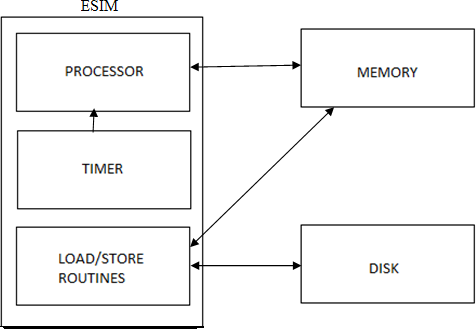
\includegraphics[scale=0.5]{pics/components_machine}
	\caption{Components of the Machine}
	\label{fig:components}
\end{figure}

The various components of the machine are :
\begin{itemize}
	\item \textbf{Disk :} It is a non-volatile storage that stores user programs (executables) and data files. \index{Disk}
	\item \textbf{Memory :} It is a volatile storage that stores the programs to be run on the machine as well as the operating system that manages the various programs. \index{Memory}
	\item \textbf{Processor :} It is the main computational unit that is used to execute the instructions. \index{Processor}
	\item \textbf{Timer :} It is a device that interrupts the processor after a pre-defined specific time interval. \index{Timer}
	\item \textbf{Load/Store :} It is a macro that performs the functionalities of \emph{DMA controller} \index{Load/Store}
	\footnote{\textbf{DMA controller :} DMA (Direct Memory Access) is the hardware device in a real machine that facilitates the transfer of data from disk to the memory and vice versa}.
	% No console device i,e. input output is done through keyboard, monitor and they are not simulated.
\end{itemize}

\section{Data types}
The fundamental types supported by the machine are \textit{integer} and \textit{string}.
\index{Machine!Data Types}
A string is a sequence of characters terminated by \verb|'\0'|. The machine interprets a single character also as a string.
\begin{example}
	The character ``s'' is stored as ``s\verb|\0|'' in the memory and the word ``ESIM'' is stored as ``ESIM\verb|\0|'' in the memory.
\end{example}
\ESIM supports a maximum string length of \emph{16}.

\chapter{Registers}
\index{Registers}
\label{chp:registers}

\section{Introduction}
The \ESIM architecture maintains \textbf{12} registers each of size 1 word.
\index{Memory!Word}
\begin{defn}
	\textbf{Word :} It is the  basic unit of memory. 
\end{defn}
Each register can hold either an integer or an address of a string.

\section{Register Set}
\index{Memory!Register Set}
There are 8 \emph{General Purpose Registers}, R0--R7, which the user programs can use directly. These are followed by another 8 \emph{Kernel Registers}, S0--S7 which are used only by the kernel. There are an additional 4 \emph{Temporary Registers}, T0--T3 which are used by the compiler.\footnote{It is recommended that the programmer, system or otherwise, not use these temporary registers.} There are also 4 additional special purpose registers BP, IP, SP and PID which are used as Base pointer, Instruction pointer, Stack pointer and Process Identifier respectively.
Figure~\ref{tbl:registers} summarises the various registers and the sections where they are referred. 
\begin{figure}[h!]
	\centering
	\begin{tabular}{|c|c|m{5cm}|}
		\toprule
		\textbf{Name} & \textbf{Register} & \textbf{Section} \\
		\toprule
		General Purpose Registers & R0--R7 & Used by the user programs to store data during various operations (Refer section~\ref{sec:unprvlgd} for the operations supported). \\
		\hline
		Kernel Registers & S0--S7  & Used by the OS to store data during various operations.(Refer section~\ref{sec:prvlgd} for the operations supported). \\
		\hline
		Temporary Registers & T0--T3 & Used by the translator for storing intermediate data. \\
		\hline
		Stack Pointer & SP & Section~\ref{register details} \\ 
		\hline
		Base Pointer & BP & Section~\ref{register details} \\ 
		\hline
		Instruction Pointer & IP & Section~\ref{register details} \\ 
		\hline
		Process Identifier & PID & Section~\ref{register details} \\
		\bottomrule
	\end{tabular}
	\caption{Summary of the registers in \ESIM architecture}
	\label{tbl:registers}
\end{figure}
\chapter{Memory}
\label{chp:memory}
\index{Memory}

\section{Introduction} 
\index{Memory!Structure}

\newcommand{\memoryLayout}[1]
{

	\begin{figure}[htp!] \small
		\centering
		\begin{tabular}{|c|c|c|}
			\toprule
			\textbf{Page no} & \textbf{Contents} & \textbf{Word addr} \\
			\toprule 
			0   & \hyperref[lbl:romcode]{ROM code} 		& 0 -- 255 \\ \hline 
			1   & \hyperref[lbl:oscode]{OS Startup code} 	& 256 -- 511  \\ \hline 
			\multirow{5}{*}{2} 
				& \hyperref[lbl:pgtbl]{Static Page Tables}   & 512 -- 559 \\ \cline{2-3} 
				& \hyperref[lbl:memlst]{Memory Free List}  & 560 -- 623  \\ \cline{2-3}
				& \hyperref[lbl:gft]{Global File Table}  & 624 -- 719 \\ \cline{2-3}
				& \hyperref[lbl:rdylst]{Ready List} & 720 -- 731 \\ \cline{2-3}
				& Unallocated & 732 -- 767 \\ \hline 
			\multirow{2}{*}{3}
				& \hyperref[lbl:proctbl]{Process Table} & 768 -- 959 \\ \cline{2-3}
				& Unallocated & 960 -- 1023 \\ \hline 
			4 & \multirow{2}{*}
				{\hyperref[lbl:fat]{File Allocation Table}} & \multirow{2}{*}{1024 -- 1535} \\ \cline{1-1} 
			5 & 				 &  \\ \hline 
			6 & \multirow{2}{*}
				{\hyperref[lbl:disklst]{Disk Free List}} & \multirow{2}{*}{1536 -- 2047}\\ \cline{1-1} 
			7 & 				& \\ \hline 
			8 & \multirow{3}{*}
				{\hyperref[lbl:INITprocess]{INIT process}} & \multirow{3}{*}{2048 -- 2815} \\ \cline{1-1} 
			9 & 				 &  \\ \cline{1-1} 
			10 & 				 &  \\ \hline 
			\multirow{3}{*}{11 -- 55}
				&  \vdots & \\   
				&  User Programs & 2816 -- 14335 \\  
				& \vdots & \\ \hline 
			56 & \hyperref[lbl:int]{INT 0} & 14336 -- 14591 \\ \hline 
			57 & \hyperref[lbl:int]{INT 1} & 14592 -- 14848 \\ \hline 
			\vdots & \vdots & \vdots \\ \hline 
			63 & \hyperref[lbl:int]{INT 7} & 16128 -- 16383 \\  
			\bottomrule
		\end{tabular}
		\caption{Outline of the main memory}
		\label{#1}
		\index{Memory!Structure}
	\end{figure}

}

\memoryLayout{fig:main memory}

\begin{itemize}
	\item The basic unit of memory in the \ESIM architecture is a word. \index{Memory!Word}
	\item The machine memory can be thought of as a linear sequence of words.
	\item A collection of 256 contiguous words is known as a \emph{page}. \index{Memory!Page}
	\item The total size of the memory is 64 pages or 16384 ($256 \times 64$) words.
	\item Each word in the memory is identified by the \emph{word address} in the range 0 to $16383(256 \times 64 - 1)$. Similarly, each page in the memory is identified by the \emph{page number} \index{Memory!Page number} in the range 0 to 63.
\end{itemize}

\begin{example}
	The $256^{th}$ word of the memory has a word address 255 and belongs to page 0. In general, the $n^{th}$ word has the word address $(n-1)$, where  $1 \le n \le 16384$ and belongs to the page $\lfloor \frac{n-1}{256} \rfloor$. Refer figure~\ref{fig:mem_struct}. 
\end{example}

\begin{figure}[htp!] \small
	\centering
	\begin{tabular}{c|c|c|} 
		\multicolumn{3}{c}{} \\
		\textbf{Word address} &  & \textbf{Page no.} \\ \cline{2-3}
		0 & $1^{st}$ word & \multirow{4}{*}{$0$} \\ \cline{2-2}
		1 & $2^{nd}$ word &  \\ \cline{2-2}
		\vdots & \vdots & \\ \cline{2-2}
		255 & $256^{th}$ word &  \\ \cline{2-3}
	
		\vdots & \vdots & \multirow{2}{*}{$\lfloor \frac{i}{256} \rfloor $} \\ \cline{2-2}
		$i$ & $(i+1)^{th} $ word &  \\ \cline{2-2}
		\vdots &\vdots &  \\ \cline{2-3}
	
		\vdots & \vdots & \multirow{2}{*}{$63$} \\ \cline{2-2}
		\vdots &\vdots &  \\ \cline{2-2}
		$256 \times 64 - 1$ & $(256 \times 64)^{th} $ word &  \\ \cline{2-3}
	\end{tabular}
	\caption{Illustration of memory addressing}
	\label{fig:mem_struct}
\end{figure}

\section{Page Table}
\index{Page Table}

Before explaining the page table, we explain two well known terms:
\begin{itemize}
	\item \textbf{Logical address :} It is the CPU generated address of the data. 
	\item \textbf{Physical address :} It is the exact location of the data in the main memory.
\end{itemize}

\begin{figure}[h!]
	\centering
	\includegraphics[scale=0.55]{pics/paging}
	\caption{Paging model of the \ESIM architecture}
	\label{fig:paging}
	\index{Page Table!Paging Model}
\end{figure}

Refer ``Memory management strategies" in the book \cite{galvin} to know more about paging. 

The page table contains information relating to the actual location in the memory, i.e., the physical address, of the data specified by the logical address. Each entry of a page table contains the page number in the memory where the data specified by the logical address resides. Refer figure~\ref{fig:paging}.


\section{Address Translation} 
\index{Address Translation}
It is the process of obtaining the physical address from the logical address. It is done by the machine in the following way. Refer book~\cite{Bach} for more details.

\begin{enumerate}
	\item The logical address generated by the CPU is divided by the page size (256) to get the \emph{logical page number}.
	\item The remainder got after performing the above division gives the \emph{offset} within that page.
	\item The \emph{logical page number} is then used to index the page table to get the corresponding \emph{physical page number} in the memory.
	\item The \emph{offset} got in step 2 is then used to refer to the word in the physical page containing the data.\\
\end{enumerate}

\begin{figure}[h!]
	\centering
	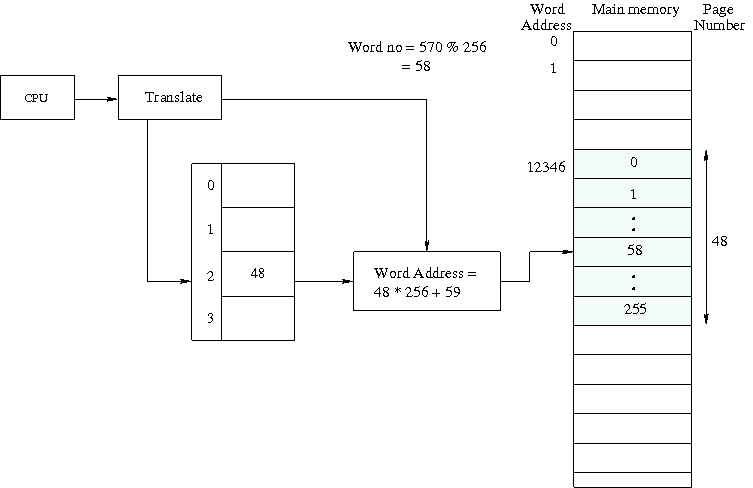
\includegraphics[scale=0.55]{pics/paging_example}
	\caption{Diagram illustrating address translation}
	\label{fig:paging_example}
\end{figure}

\begin{example}
	Consider the scenario in figure~\ref{fig:paging_example}. Here the logical address generated is 570, so the page number is $ \lfloor 570/265 \rfloor = 2$ and word address is $570\mbox{ mod }256 = 58$. The looked up value from the page table is $48$. Thus the resultant physical address is $48 \times 256+58$.
\end{example}
	
\section{Memory Free List}
\label{lbl:memlst}
\index{Memory!Free list}

\begin{itemize}
	\item The free list of the memory consists of 64 entries. Each entry is of size one word.
	\item The total size of the free list is thus 64 words (64 (= no. of entries) $\times$ 1 (= size of one entry) = 64 words).
	\item It is present in the second 64 words of page 2 of the memory. Refer figure~\ref{fig:main memory}.
	\item Each entry of the free list contains a value of either 0 or 1 indicating whether the corresponding page in the memory is free or not respectively.
\end{itemize}

\begin{example} 
	Figure~\ref{fig:mem_free_list} indicates that pages 0, 1 and 63 of the memory are not free while pages 2 and 48 are free.
\end{example}

\begin{figure}[htp!] \small
	\centering
	\begin{tabular}{c|c|}
%		\multicolumn{2}{c}{} \\ 
		\textbf{Pg no.} & \textbf{Contents} \\ \cline{2-2}
		$0$ & $1$ \\ \cline{2-2}
		$1$ & $1$ \\ \cline{2-2}
		$2$ & $0$ \\ \cline{2-2}
		\vdots & \vdots \\ \cline{2-2}
		$48$ & $0$ \\ \cline{2-2}
		$\vdots$ & \vdots \\ \cline{2-2}
		$63$ & $1$ \\ \cline{2-2}
	\end{tabular}
	\caption{A sample free list of the memory}
	\label{fig:mem_free_list}
\end{figure}

The entire structure of memory is outlined in figure~\ref{fig:main memory}.

\chapter{Process}
\label{chp:process}
\index{Process}

\section{Introduction}
\begin{defn}
	\textbf{Process :} Any program written by the user is run as a process by the kernel. 
\end{defn}
\begin{itemize}
	\item The {\ESIM} architecture supports a maximum of 12 processes to be run at a time.
	\item Each process occupies 4 pages of the memory.
\end{itemize}

\section{Process Structure}
\index{Process!Structure}
A process in the memory has the following structure.
\begin{itemize}
	\item \textbf{Code Area :} \index{Process!Code Area} These are pages of the memory that contain the actual code to be run on the machine. It occupies 2 pages of the memory. 
	\item \textbf{Data Area :} \index{Process!Data Area} This section consists of string data that is used in the code which cannot be stored in a register. It occupies 1 page of the memory.
	\item \textbf{Stack :} This is the user stack used in program execution. It is used to pass arguments during function calls, storing activation record of a function etc.  It occupies 1 page of the memory and grows in the direction of increasing word address.
\end{itemize}

Figure~\ref{fig:process structure} shows the process structure. \\

\begin{figure}[htp!] 
	\centering
	\begin{tabular}{|c|c} 
		\textbf{Contents}     & \textbf{Pg no:} \\ \cline{1-1}
		\multirow{2}{*}{Code} & $0$ \\
				      & $1$ \\ \cline{1-1}
		Data & 2 \\ \cline{1-1}
		\noalign{\smash{\llap{\lower2pt\hbox{\tt BP$\longrightarrow$}}}}
		&  \\
		&  \\
		\noalign{\smash{\llap{\raise2pt\hbox{\tt $\bigg \downarrow$ }}}}
		Stack & 3 \\ \cline{1-1}
		\noalign{\smash{\llap{\lower2pt\hbox{\tt SP$\longrightarrow$}}}}
	\end{tabular}
	\caption{Process Structure in memory. Arrow shows the direction of stack growth}
	\label{fig:process structure}
\end{figure}

\section{Registers Associated with a Process}
\label{register details}
\begin{itemize}
	\item Every process is allotted a unique integer identifier in the range 0 to 11, known as the PID (Process Identifier) which is stored in the PID register. This register can be used as an operand in any instruction only when executing in the kernel mode. (Refer section~\ref{sec:modes} to know about the modes of operation)
	\index{Registers!PID}
	\item The word address of the currently executing instruction is stored in the IP (Instruction Pointer) register. This register can be used as an operand in any instruction only when executing in the kernel mode.
	\index{Registers!IP}
	\item The base address of the user stack is stored in the BP (Base Pointer) register. \index{Registers!BP}
	\item The address of the stack top is stored in the SP (Stack Pointer) register. \index{Registers!SP}
\end{itemize}
Each process has its own set of values for the various registers.

\section{Data Structures Associated with a Process}
\index{Process Data Structures}

The following are the various data structures associated with a process. They are explained in the following subsections.

\subsection{Ready List}
\index{Process!Ready List}
\label{lbl:rdylst}
The \textit{ready list :} is the data structure that maintains a circular list of all the active processes. Each entry of the ready list contains a value of either 1 or 0 indicating whether the corresponding process in the memory is present in the list or not.

\subsection{Process Control Block (PCB)}
\label{sec:pcb}
\index{Process Data Structures!Process Control Block}
It contains data pertaining to the current state of the process. Refer figure~\ref{fig:PCB}.\\

\newcommand{\pcb}[1]{
	\begin{figure}[htp!]
		\centering
		\begin{tabular}{|c|c|c|c|c|c|}
			\hline
			0 & 1 & 2 & 3 & 4--11 & 12--15 \\
			\hline
			PID & BP & SP & IP & R0 -- R7 & Local File Table \\
			\hline
		\end{tabular}
		\caption{Structure of Process Control Block}
		\label{#1}
	\end{figure}
	}

\pcb{fig:PCB}

Note that the size of each PCB (Process Control Block) is 16 words. 

\subsection{The Page Table}
\label{lbl:pgtbl}
\index{Process!Page Table}
The \emph{page table} stores the exact location in the memory of the data related to a process.
\begin{itemize}
	\item Each process has 4 entries in the page table.
	\begin{itemize}
		\item The zeroth entry corresponds to the first page of code area.
		\item The first entry corresponds to the second page of code area.
		\item The third entry corresponds to the data area.
		\item The fourth entry corresponds to the stack.
	\end{itemize}
	\item Each entry contains the page number where the data specified by the logical address resides in the memory. Refer figure~\ref{fig:paging}.
\end{itemize}

\section{Storage Details of the Data Structures}
	The data structures used by the processes are stored statically in the memory. Their storage details are as follows.\\

\begin{figure}[htp!]
	\centering
	\subfigure[Main Memory]{
	\renewcommand{\arraystretch}{1.2}
	\scalebox{0.85}{
	\begin{tabular}{r|c|} \small
		\textbf{Pg no.} & \textbf{Contents} \\ \cline{2-2}
		0   &  \\ \cline{2-2}
		1   &  \\ \cmidrule{2-2}
		\multirow{4}{*}{2}
			& \cellcolor{gray!70} Static Page Tables   \\ \cline{2-2}
			& Memory Free List     \\ \cline{2-2}
			& Global File Table    \\ \cmidrule{2-2}
			& \cellcolor{cyan!70} Ready List  \\ \cline{2-2}
		3   & \cellcolor{orange!70} Process Table  \\ \cline{2-2}
		    & \vdots \\ \cline{2-2}
		7  &  \\ \cline{2-2}
		\multirow{3}{*}{8 -- 55}
			&  \vdots  \\
			&  User Programs \\
			& \vdots  \\ \cline{2-2}
			&  \\ \cline{2-2}
		56 -- 63 & INT 0 -- 7  \\ \cline{2-2}
		& \vdots   \\ \cline{2-2}
	\end{tabular}}} \\

	\subfigure[Structure of Page Table]{
	\renewcommand{\arraystretch}{1.2}
	\scalebox{0.7}{
	\begin{tabular}{|>{\columncolor[gray]{.8}}c|m{1cm}} \small
		Word Address & Process  \\
		0 & \multirow{4}{*}{$0$}  \\
		1 &  \\
		2 &  \\
		3 &  \\ \cmidrule{1-1}
		\vdots &  \\ \cmidrule{1-1}
		$4i$ & \multirow{4}{*}{$i$}  \\ \cline{1-1}
		$4i+1$ &  \\
		$4i+2$ &  \\
		$4i+3$ &  \\ \cmidrule{1-1}
		\vdots &  \\ \cmidrule{1-1}
		$44$ & \multirow{4}{*}{$11$}  \\
		$45$ &  \\
		$46$ &  \\
		$47$ &  \\
	\end{tabular}}} \qquad \qquad
	\subfigure[Structure of Ready List]{
	\renewcommand{\arraystretch}{1.2}
	\scalebox{0.7}{
	\begin{tabular}{|>{\columncolor{cyan}}c|m{1cm}} \small
		Word Address & Process  \\
		0 & $0$ \\
		1 & $1$ \\
		2 & $2$ \\
		\vdots &  \\
		10 & $10$ \\
		11 & $11$ \\
	\end{tabular}}} \qquad \qquad
	\subfigure[Structure of Process Table]{
	\renewcommand{\arraystretch}{1.2}
	\scalebox{0.7}{
	\begin{tabular}{|>{\columncolor[rgb]{1,0.5,.1}}c|m{1cm}} \small
		Word Address & Process  \\
		0 & \multirow{4}{*}{$0$}  \\
		1 &  \\
		\vdots &  \\
		15 &  \\ \cmidrule{1-1}
		\vdots &  \\ \cmidrule{1-1}
		$16i$ & \multirow{4}{*}{$i$}  \\
		$16i+1$ &  \\
		$16i+2$ &  \\
		\vdots & \\
		$16i+15$ &  \\ \cmidrule{1-1}
		\vdots &  \\ \cmidrule{1-1}
		$176$ & \multirow{4}{*}{$11$}  \\
		$177$ &  \\
		\vdots &  \\
		$191$ &  \\
	\end{tabular}}} \\
	\caption{Data Structures associated with a process}
	\label{fig:ds with process}
\end{figure}

\subsection{Ready List}
\begin{itemize}
	\item The ready list is located in words 209--220 of page 2 of the memory (refer fig~\ref{fig:main memory}).
	\item The size of each ready list entry is one word.
	\item There are a total of 12 processes, thus accounting for the 12 words (12 $\times$ 1 word).
	\item All active processes have an entry 1 in the ready list corresponding to the location indexed by their respective PIDs.
\end{itemize}

\subsection{Page Tables}
\begin{itemize}
	\item The page tables of the 12 processes are stored in the first 48 words of page 2 of the memory. Refer figure~\ref{fig:main memory}.
	\item The size of each page table is 4 words ( 4(= no. of entries) $\times$ 1(= size of an entry)= 4 words).
	\item There are a total of 12 processes, thus accounting for the 48 words( 12 $\times$ 4 words).
	\item The page tables are indexed by multiplying the PID of a process by the size of a page table to get the starting word address of the page table of that process.  The indexing mechanism is illustrated in figure~\ref{fig:ds with process}.
\end{itemize}

\subsection{Process Table}
\index{Process!Process Table}
\label{lbl:proctbl}
\begin{itemize}
	\item The page 3 of the memory contains the process table. Refer figure~\ref{fig:main memory}.
	\item The process table contains the PCB of each of the 12 processes (Each entry occupies 16 words).
	\item There are a total of 12 processes, thus accounting for the 192 words (12 $\times$ 16 words).
	\item The process table is indexed by multiplying the PID of a process by the size of a PCB to get the starting word address of the PCB of that process. The indexing mechanism is illustrated in figure~\ref{fig:ds with process}.
\end{itemize}

\chapter{Instructions}
\label{chp:instr}
\index{Instructions}

\section{Introduction}
All instructions in the SIM architecture are present in the \ESIM architecture as well. The additional instructions provided by the \ESIM architecture can be classified into \emph{privileged} and \emph{unprivileged} instructions (Refer to the ~\href{http://www.athena.nitc.ac.in/~kmurali/Compiler/sim.html}{SIM manual} for the  instruction set and addressing modes). % TODO Give reference to appendix.

\section{Processor Modes}
\label{sec:modes}
\index{Processor!Modes}
The ESIM architecture is interrupt driven and uses a single processor. There are two modes of operation, the user mode and the kernel mode.
\begin{itemize}
	\item \textbf{User mode :} All unprivileged instructions can be executed in this mode. 
	\item \textbf{Kernel mode :} Both privileged and unprivileged instructions can be executed in this mode. Initially, the machine starts in kernel mode.
\end{itemize}

The processor comes to know about the mode in which the system is running by looking at the value in the IP register.

\section{Classification}
\subsection{Unprivileged Instructions}
\label{sec:unprvlgd}
\index{Instructions!Unprivileged}
All the instructions in the SIM architecture except the HALT instruction constitute the unprivileged instructions. In addition to that, we have five more instructions in the \ESIM architecture, one interrupt service instruction and four instructions for string operations. They are:
\begin{enumerate}
	\item \texttt{INT} \\ Syntax : INT \emph{no} \\
	This instruction generates an interrupt to the kernel with \emph{no} as a parameter. It pushes the current IP+1 value into the stack and switches the machine from \textit{User mode} to \textit{Kernel mode}. The address of the first instruction of the specified ISR is stored into the IP register. Execution is started at the address specified IP. Refer section~\ref{interrupts} to know more about interrupts.
	
	\item \texttt{SIN Rn} - This instruction is used to take strings as input. The input string is stored in the data section of the program at the logical address specified by the value in Rn.
	
	\item \texttt{SOUT Rn} - This instruction prints the string stored at the logical address specified by the value in Rn. Figure~\ref{sout example} illustrates this instruction.

	\begin{figure}[htp!]
	\centering
	\subfigure[Code Section]{
	\renewcommand{\arraystretch}{1.2}
	\scalebox{0.75}{
	\begin{tabular}{|r|c|} \small
	0 & \texttt{MOV R1 512} \\ \cline{2-2}
	1 & \texttt{SOUT R1} \\ \cline{2-2}
	2 & \texttt{MOV R1 513} \\ \cline{2-2}
	3 & \texttt{SIN R1} \\ \cline{2-2}
	4 & \texttt{SOUT R1} \\ \cline{2-2}
	\vdots & \vdots \\ \cline{2-2}
	255 & \ldots \\ \hline \hline
	256 & \ldots \\ \cline{2-2}
	\vdots & \vdots  \\ \cline{2-2}
	511 & \ldots \\  \hline
	\end{tabular}}} \\
	\subfigure[Data Section: initial contents]{
	\renewcommand{\arraystretch}{1.2}
	\begin{tabular}{|r|c|} \small
	512 & \texttt{HELLO$\backslash$0} \\ \cline{2-2}
	513 & \ldots \\ \cline{2-2}
	\vdots & \vdots \\ \cline{2-2}
	767 & \ldots \\ \hline
	\end{tabular}} \qquad
	\subfigure[Data Section: after execution of \texttt{SIN} instruction]{
	\renewcommand{\arraystretch}{1.2}
	\begin{tabular}{|r|c|} \small
	512 & \texttt{HELLO$\backslash$0} \\ \cline{2-2}
	513 & \texttt{ESIM$\backslash$0} \\ \cline{2-2}
	\vdots & \vdots \\ \cline{2-2}
	767 & \ldots \\ \hline
	\end{tabular}} \qquad \qquad
	\subfigure[]{
	\begin{tabular}{c}
	\textbf{\underline{Output}} \\
	\texttt{HELLO} \\
	\texttt{512} \\
	\texttt{ESIM}
	\end{tabular}}
	\caption{Example for \texttt{SOUT} instruction}
	\label{sout example}
	\end{figure}

	\item \texttt{STRCPY Ri Rj} - This instruction copies the string stored in 
	the data section at the logical address specified by the register Rj to 
	the logical address specified by the register Ri.
	\item \texttt{STRCMP Ri Rj} - This instruction compares the strings stored in 
	the data section at the logical addresses specified by the registers Ri and Rj and returns a 
	value 0 if the strings are equal and -1 otherwise. The returned value is stored in Ri.
	\end{enumerate}
	
\subsection{Privileged Instructions}
\label{sec:prvlgd}
\index{Instructions!Privileged}
There are \emph{four} privileged instructions. These instructions can be executed only in kernel mode. They are:
\begin{itemize}
	\item \texttt{IRET} \\
	Syntax : IRET \\
	IRET tells the processor that the interrupt handler has finished. This instruction pops the return address of the process from the stack into the IP register and switches the machine from kernel mode to user mode.
	Refer section ~\ref{interrupts} to know more about the IRET instruction.
	
	\item \texttt{LOAD} \index{Load/Store} \footnote{These are macros which initialise the DMA controller with the arguments passed and invoke it for the actual transfer to take place.}
	\\ Syntax : LOAD \emph{pg\_no} \emph{block\_no} \\
	This instruction loads the block specified by the  \emph{block\_no}, from the disk, to the page specified by the  \emph{pg\_no}, in the memory.
	
	\item \texttt{STORE$^{1}$} \index{Load/Store} \\
	Syntax : STORE \emph{block\_no} \emph{pg\_no} \\ 
	This instruction stores the page specified by the \emph{pg\_no}, from the memory, to the block specified by the \emph{block\_no}, in the disk.
	
	\item \texttt{HALT} \\
	Syntax : HALT \\
	This instruction causes the simulator to halt immediately.
\end{itemize}

	%TODO Add details on how modes are detected 
	%Refer chapter~\ref{chp:memory} for more details.
	% TODO Give references to appropriate sections. Why to give refs here? Also do clean up by moving infos to restriction section.

\chapter{Interrupts}
\label{chp:int}
\index{Interrupts}
\label{lbl:int}

\section{Introduction}
Interrupts are mechanisms by which the user code interrupts the execution of the processor and passes control to the kernel to accomplish low level functionalities like disk access, arithmetic exception handling etc.

\textbf{Interrupt Service Routine(ISR)} : The kernel provides routines to accomplish the functionality for which an interrupt has been generated. These routines are known as Interrupt Service Routines. \index{Interrupts!Interrupt Service Routine}

\textbf{Note: } Every ISR should end with an IRET instruction.

\section{The \texttt{INT} instruction}
\label{interrupts}
The instruction used to generate an interrupt is \texttt{INT}. \\ Syntax : \texttt{INT} \emph{n} 

The INT instruction passes control to the Interrupt Service Routine (ISR) for this interrupt located at the physical address 
computed using the value n.

Address computation is done as follows. 
The physical address of the ISR corresponding to interrupt number $n$ is given by:
\begin{equation*} 
\mbox{Physical Address} = (56+n) \times \mbox{Page Size}
\end{equation*}

\index{Interrupts!Table}
Figure~\ref{interrupt table} summarises the physical address to which the control is transferred for each interrupt. Note that the interrupts are disabled once this instruction is executed, since we do not allow interrupts to occur in kernel mode.

\begin{figure}[htp!]
	\centering
	\renewcommand{\arraystretch}{1.2}
	\begin{tabular}{cccc}
		\toprule
		Interrupt No. & \multicolumn{3}{c}{Word Address} \\ \cline{2-4}
		& Page No. & Offset & Address \\ \midrule
		0 & 56       & 0      & $56\times256+0$=$14336$ \\
		1 & 57       & 0      & $57\times256+0$=$14592$ \\
		2 & 58       & 0      & $58\times256+0$=$14848$ \\
		3 & 59       & 0      & $59\times256+0$=$15104$ \\
		4 & 60       & 0      & $60\times256+0$=$15360$ \\
		5 & 61       & 0      & $61\times256+0$=$15616$ \\
		6 & 62       & 0      & $62\times256+0$=$15872$ \\
		7 & 63       & 0      & $63\times256+0$=$16128$ \\
		\bottomrule
	\end{tabular}
	\caption{Interrupts and their locations in the memory}
	\label{interrupt table}
\end{figure}

\memoryLayout{fig:main memory8}

\section{Types of Interrupts}
\index{Interrupts!Types}
There are 8 interrupts (numbered from 0 to 7) supported by the {\ESIM} architecture. The interrupts 0 is a hardware interrupts and the remaining interrupts (1 to 7) are software interrupts.\\

Details of the \emph{hardware interrupt} is as follows.

\begin{itemize}
	\item \texttt{INT 0 :} This is the timer interrupt \index{Timer} which interrupts the processor forcing a context switch. It contains the code for the scheduler of the operating system (refer section~\ref{chp:scheduler}), which schedules the CPU time among the various active processes. Note that this interrupt is machine generated and cannot be called.
%	\item \texttt{INT 7 :} It is generated when the following exceptions\footnote{An exception is an abnormal condition that arises when the machine deviates from its normal execution pattern.} occur:
%	\begin{enumerate}
%		\item \emph{Illegal memory access :} occurs when any address generated by the process does not
%		lie in the range [0, 959].
%		\item \emph{Arithmetic exception :} occurs when divisor is 0.
%		\item \emph{Illegal instruction :} occurs when an attempt is made to execute an instruction not belonging to the instruction set and also when the operands to the instruction is not legal. Eg: \texttt{MOV 4 R0}, \texttt{MOV IP 4} when executed in user mode. These instructions are considered illegal.
%		\item \emph{Stack overflow and stack underflow :} Stack overflow occurs when the value in the SPregister exceeds 959 and stack underflow occurs when the value falls below 768.
%	\end{enumerate}
\end{itemize}
%Refer chapter~\ref{chp:exception} for to know more about the way exceptions are handled.

Details of \emph{software interrupts} are as follows.
\begin{itemize}
	\item \texttt{INT 1--4:} These interrupts are used for the various file system calls. (Refer section~\ref{fssyscall} for File System Calls)
	\item \texttt{INT 5--7:} These interrupts are used for the various process system calls. (Refer section~\ref{procsyscall} for Process System Calls)
\end{itemize}
The interrupts 1--7  are unprivileged and can be called from user mode.

% TODO Should explain how interrupts are serviced ? i,e. give some assembly code ? Probably can be given in appendix.

\section{Calling Convention}
\label{callconv}
\index{Calling Convention}
In this section, we explain the calling and returning conventions for interrupts.\footnote{The convention given above is already built into the AP-SIL compiler. It has been given only to help you understand the internal workings better.}

\subsection{Calling Convention}
Before switching the control to the ISR using the INT instruction the user program does the following:
\begin{enumerate}
	\item Push a dummy value for storing the return value of the interrupt onto the stack.
	\item Push the arguments to the interrupt.
	\item Make the Interrupt call using the INT instruction.
\end{enumerate}

The INT instruction pushes the IP+1 value on to the stack and then starts the execution of the corresponding ISR. When the ISR finishes its execution, IRET instruction is called. This IRET instruction pops the IP+1 value from the stack top into the IP register and the execution of the user program is resumed from the point where it was interrupted.

\subsection{Returning Convention}
After returning from the ISR using the IRET instruction the user program does the following:
\begin{enumerate}
	\item Pop out the arguments from the stack.
	\item Pop out the return value.
\end{enumerate}

Figure~\ref{fig:calling_convention} explains the state of the stack at various stages.

\begin{figure}[htp!]
	\centering
	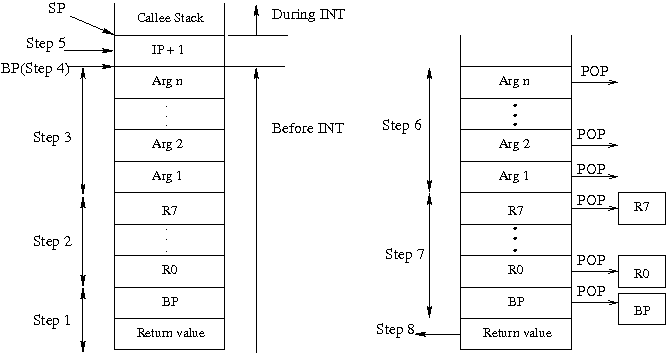
\includegraphics[scale=0.55]{pics/calling_convention}
	\caption{Recommended calling and returning convention for interrupts}
	\label{fig:calling_convention}
\end{figure}


\part{Machine Implementation}
\chapter{Machine Implementation}
\label{chp:machImplmnt}

\section{Machine}
The implementation details for the machine are given below. details given include the header file, the corresponding code file, the various functions included in them and a short description of these functions.

\begin{enumerate}
	\item \textit{data.h }
	
	Consists of constants declared for the machine. These include the registers, and the size of various constiuents of memory. The entire memory is declared here as well.
	
	\item \textit{memoryConstants.h}
	
	Declarations for the structure of main memory is made here.
	
	\item \textit{instr.h}
	
	Declares the constants associated with each token.
	
	\item \textit{decode.lex}
	
	This is the lexical analyser which analyses each instruction and reurns the corresponding token.
	
	\item \textit{boot.h} and \textit{boot.c}
	
	This file consists of the following functions:
	\begin{itemize}
		\item void loadStartupCode() - Loads the OS Startup Code from disk to the proper location in memory
		\item void initializeRegs() - Initializes the values of all the registers to zero.
	\end{itemize}
	
	\item \textit{scheduler.h} and \textit{scheduler.c}
	
	This file consists of the following functions:
	\begin{itemize}
		\item void runInt0Code() - Causes the timer interupt leading to the control being passed on to the INT 0 code in memory.
	\end{itemize}

	\item \textit{timer.h}
	
	This file contains the constant defining the number of clock cycles that makes up a timslice alloted to a single process. This file also consists of the following functions:
	\begin{itemize}
		\item int isTimeZero() - Checks whether the timer counter reads zero.
		\item void tick() - Decrements the timer counter.
		\item void resetTimer() - Resets the timer counter.
	\end{itemize}
	
	\item \textit{utility.h} and \textit{utility.c}
	
	This file consists of the following functions:
	\begin{itemize}
		\item void emptyPage(int) - Clears the page speecified by the aguement.
		\item struct address translate(int) - Translates the virtual address passed as arguement to the corresponding page number and offset.
		\item printRegisters() - Prints the values of all the registers. Used for debugging purposes.
		\item void exception(char*) - Acts as the exception handler. Prints the instruction that caused the exception and terminates execution.
	\end{itemize}

	\item \textit{simulator.h} and \textit{simulator.c}

	This file consists of the following functions:
	\begin{itemize}
		\item void Executeoneinstr(int) - This function simulates all the instructions available on the esim architecture. 
		\item void run(int, int) - This function acts as the bootloader. It loads the Startup code. It also calls Executeoneinstr() for every instruction that it reads.
		\item int main(int, char**) - Makes the initial changes to the machine environment and the calls run().
	\end{itemize}

\end{enumerate}

\part{File System Specification}
\chapter{File System}
\label{chp:fs}

\section{Introduction}
\index{Block}
\begin{defn}
	\textbf{Block :} It is the basic unit of storage in the disk.
\end{defn}
	
The disk can be thought of as consisting of a linear sequence of 512 blocks.
The size of each block is equal to that of a page in the memory (256 words). 

\section{Disk Structure}
\index{Disk!Structure}
The basic structure of the disk is shown in figure~\ref{fig:disk}.

\begin{figure}[htp!] \small
	\centering
	\begin{tabular}{|c||c|c|c|c|c|c|c|c|}
		\hline
		\textbf{Block No.} & 0 & 1 & 2 & \ldots & 8 & 9--10 & 11--12 & 13--511 \\ \hline
		\textbf{Contents} & OS Startup code & INT 0 & INT 1 & \ldots & INT 7 & Free List & FAT & Data Blocks \\ \hline
	\end{tabular}
	\caption{Structure of the disk}
	\label{fig:disk}
\end{figure}

\section{Addressing}
\index{Disk!Addressing}
\begin{defn}	
	\textbf{Block number :} Any particular block in the disk is addressed by the corresponding number in the sequence 0 to 511 known as the \emph{block number}.
\end{defn}

\begin{figure}[htp!] 
	\centering
	\scalebox{0.85}{
	\begin{tabular}{|c|c|c|}
		\toprule
		\textbf{Block} & \textbf{Contents} & \textbf{Block no.} \\ \toprule
		\multirow{4}{*}{$1$} & $0^{th}$ word & \multirow{4}{*}{$0$} \\
					  &  $1^{st}$ word &  \\
					  &  \vdots &   \\
					  &  $255^{th}$ word &  \\ \hline
		\multirow{4}{*}{$2$} &  $256^{th}$ word &  \multirow{4}{*}{$1$} \\
					  &  $257^{th}$ word &   \\
					  &  \vdots &  \\
					  &  $511^{th}$ word &  \\ \hline
		\vdots & \vdots & \vdots \\ \hline
		\multirow{3}{*}{$512$} & \vdots & \multirow{3}{*}{511}   \\
					    & \vdots &  \\
					    &  $(256 \times 512 - 1)^{th}$ word &  \\ \bottomrule
	\end{tabular}}
	\caption{Disk addressing}
	\label{fig:disk addr}
\end{figure}

\begin{example}
	In figure~\ref{fig:disk addr}, the $2^{nd}$ block of the disk has a block number 1. In general the $i^{th}$ block has the block number $(i-1)$ for $1 \le n \le 512$. 
\end{example}

\section{Disk Free List}
\index{Disk Free List}
\label{lbl:disklst}
\begin{itemize}
	\item  The Free List of the disk consists of 512 entries. Each entry is of size one word.
	\item  The total size of the free list is thus 2 blocks or 512 words (512(= no. of entries) $\times$ 1(= size of one entry) = 512 words).
	\item  It is present in blocks 9 and 10 of the disk. Refer figure~\ref{fig:disk}. \index{Disk!Free List Location}
	\item  Each entry of the free list contains a value of either 0 or 1 indicating whether the corresponding block in the disk is free or not respectively (It should be ensured that the first 13 entries are always marked used).
\end{itemize}
\begin{example}
	Figure~\ref{fig:disk free list} indicates that the blocks 0, 1 and 511 of the disk are not free while blocks 2 and 48 are free.
\end{example}

\begin{figure}[htp!] \small
	\centering
	\begin{tabular}{|c|c|}
		\multicolumn{2}{c}{} \\ \toprule
		\textbf{Index} & \textbf{Content} \\ \toprule
		$0$ & $1$ \\ \hline
		$1$ & $1$ \\ \hline
		$2$ & $0$ \\ \hline
		\vdots & \vdots \\ \hline
		$48$ & $0$ \\ \hline
		$\vdots$ & \vdots \\ \hline
		$511$ & $1$ \\ \hline
	\end{tabular}
	\caption{A sample free list of the disk}
	\label{fig:disk free list}
\end{figure}

\section{File}
A file \index{File} is a collection of data identified by a name. Every file in the disk has a \textit{Basic Block} and several \textit{Data Blocks}. They are defined as follows:
\begin{itemize}
	\item \textbf{Data Blocks :}  These blocks contain the actual data of a file. \index{File!Data Block}
	\item \textbf{Basic Block :}  It consists of information about the data of a file. \index{File!Basic Block}
% 	 	the location of the data blocks of the file in the disk etc.  	
	\begin{itemize}
		\item The basic block structure is shown in figure~\ref{fig:basic block}. \index{File!Basic Block Structure}
		\begin{figure}[h]
			\centering
			\begin{tabular}{|c|c|c|}
				\hline
				\textbf{Index} & 0--127 & 128--255\\
				\hline
				\textbf{Content} & Block List & Header\\
				\hline
			\end{tabular}
			\caption{Structure of the basic block of a file}
			\label{fig:basic block}
		\end{figure}
		\item The basic block consists of the \textit{Block List} and the \textit{Header}.
		\item \textbf{Block List :} It is similar to an index in a book which tells which chapter starts from which page.
		\begin{itemize}
			\item The block list consists of 128 entries.
			\item Each entry is of size one word.
			\item The size of the block list is thus 128 words (128(= no. of entries) x 1(= size of an entry) = 128 words).
			\item The value contained in an entry of the block list gives the block number of the corresponding data block in the disk.
		\end{itemize}
		\item \textbf{Header :} The header contains the header information relating to the file. Currently this is unused, but at a later stage can be used to store information such as file modification date/time, author of the file etc.
	\end{itemize}
\end{itemize}

\begin{example}
	\begin{figure}[h!]
	\centering
	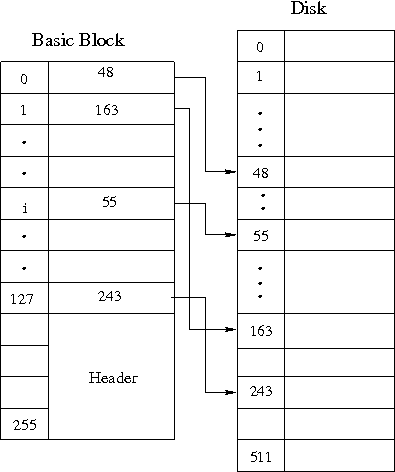
\includegraphics[scale=0.60]{pics/basic_block_example}
	\caption{Example illustrating the basic block of a file}
	\label{basic block example}
	\end{figure}

	Consider the example illustrated by figure~\ref{basic block example}.
	From the figure, we infer the following. 
	\begin{itemize}
		\item  The zeroth data block of the file resides at the disk block whose block number is 48. 
		\item  The first data block of the file resides at the disk block whose block number is 163.
		\item  The ith data block of the file resides at the disk block whose block number is 55 where $ 0\le i \le 127$. 
		\item  The 127th data block of the file resides at the disk block whose block number is 243.
	\end{itemize}
\end{example}

\subsection{File Types} 
\index{File!Types}
There are two types of files in the \ESIM architecture. They are:
\begin{enumerate}
	\item \textbf{Data files :} These files contain data or information that is used by the programs. They can occupy a maximum of 129 blocks (1 basic block + 0 - 128 data blocks).
	\item \textbf{Executable files :} These contain programs that the user wishes to run on the machine. They occupy 4 blocks (1 basic block + 3 data blocks) of the disk.
\end{enumerate}


\subsection{Executable File Format}
\index{Executable File Format}
Any executable file has the following format. Refer figure~\ref{fig:executable}.
\begin{itemize}
	\item  It consists of the \emph{Code section} and the \emph{Data section}.
	\item \textbf{Code section :} This section contains the actual code to be run on the machine. It spans 2 blocks irrespective of the size of the code.
	\index{Executable File Format!Code Section}
	\item \textbf{Data Section :} This section consists of data that is used in the code which cannot be stored in a register. The registers then store the logical address of the corresponding data residing in the data section. It spans 1 block. \index{Executable File Format!Data Section}
\end{itemize}
	
\begin{figure}[h!]
	\centering
	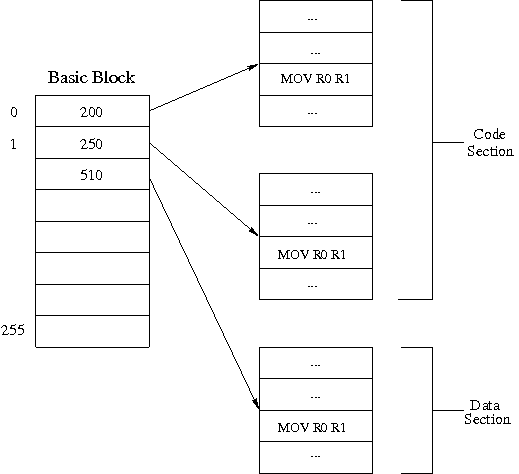
\includegraphics[scale=0.60]{pics/executable}
	\caption{Example illustrating the structure of an executable in the disk}
	\label{fig:executable}
\end{figure}

\section{File Allocation Table (FAT)}
\index{File Allocation Table}
\label{sec:fat}
\label{lbl:fat}
\emph{File allocation table} (FAT), as the name suggests, is a table that has an entry for each file present in the disk.
\begin{itemize}
	\item FAT of the filesystem consists of 32 entries. Thus there can be a maximum of 32 files. 
	\item Each entry is of size 16 words.
	\item Total size of the FAT is thus 512 words (32 (= number of entries) $\times$ 16(= size of one entry) = 512 words).
	\item It is a disk data structure and occupies block numbers 11 and 12 of the disk. Refer figure~\ref{fig:disk}. 
	\index{File Allocation Table!Location in disk}
\end{itemize}

The structure of a FAT entry is shown in figure~\ref{fig:fat_entry}. 

\begin{figure}[htp!] \small
	\centering
	\begin{tabular}{|c|c|c|c|}
		\hline
		0 & 1 & 2 & 3 -- 15 \\
		\hline
		File Name & File Size & Block no: of basic block & \dots{} Free \dots \\
		\hline
	\end{tabular}
	\caption{Structure of a FAT entry}
	\label{fig:fat_entry}
\end{figure}

The FAT entry consists of the
\index{File Allocation Table!FAT Entry}
\begin{enumerate}
	\item \textbf{File Name :} It is an identification of a file. It can be of maximum 15 characters (and thus requires 1 word). Typical file names are \texttt{student.txt}, \texttt{calc.sim}.
	\item \textbf{File size :} It indicates the number of words occupied by a file. It varies from 0 words to (128 $\times$ 256) words (depending upon the number of data blocks it has). It occupies one word in the FAT entry.
	\item \textbf{Block number of basic block :} It contains the block number where the basic block of a file resides in the disk. It occupies one word in the FAT entry.
\end{enumerate}

% \section{Restrictions}


\part{File System Implementation}
\chapter{File System Implementation}
\label{chp:fileSysImpl}

\section{File System}
The implementation details for the file system are given below. details given include the header file, the corresponding code file, the various functions included in them and a short description of these functions.
\begin{enumerate}
	\item \textit{createDisk.h} and \textit{createDisk.c} 

	This file consists of the following functions.
	\begin{itemize}
		\item void createDisk(int) : Creates a disk file if it does not exist. If it does the function also has the option of formatting the disk.
	\end{itemize}
	
	\item \textit{fileSystem.h} and \textit{fileSystem.c}
	
	The header file consists of all the constants that have been defined for implementing the filesystem. This file consists of the following functions.
	\begin{itemize}
		\item void listAllFiles() - Lists all files in the FileSystem.
		
		\item int deleteExecutableFromDisk(char*) - Deletes anexecutable file from the filesystem
		
		\item int removeFatEntry(int) - Removes the fat entry for a file.
		
		\item int getDataBlocks(int*, int) - Retrieves the datablocks for a file which already exists on the filesystem.
		
		\item int loadExecutableToDisk(char*) - Loads executable file t disk.
		
		\item int CheckRepeatedName(char*) - Checks whether a file already exists on the filesystem. If it does it returns the fat entry for that file.
		\item int FindFreeBlock() - Allocates and returns an empty block in the filesystem.
		
		\item int FindEmptyFatEntry() - Searches and returns an empty fat entry in the filesystem.
		\item void FreeUnusedBlock(int*, int) - Frees the blocks which are allocated on the disk. These are passed as the first arguement.
		
		\item void AddEntryToMemFat(int, char*, int, int) - Popuates the various fields of FAT on the disk.
		\item int writeFileToDisk(FILE*, int) - Commits the changes made to the memory copy of the file to the underlying filesystem.
		
		\item int loadOSCode(char*) - loads the Startup code onto the filesystem.
		
		\item int loadIntCode(char*, int) - loads the interrupt code code to the proper place on the filesystem depending on the arguement..
		
		\item int initializeInit() - Makes a dummy entry for init on the filesystem.
		
		\item int loadInitCode(char*) - loads init code onto the filesystem.
	\end{itemize}
	
	\item \textit{fileUtility.h} and \textit{fileUtility.c}
	
	This file consists of the following functions:
	\begin{itemize}
		\item emptyBlock(int) - Empties the memory copy of the disk
		
		\item int getInteger(char*) - Converts the arguement from char* to int and returns the int version.
		
		\item void storeInteger(char*, int) - Converts the second arguement to integer and stores it in the location specified by the first arguement. 
		
		\item int readFromDisk(int, int) - Reads an entire page from the block number specified by the second arguement to the memory location  specified by the first arguement.
		
		\item int writeToDisk(int, int) - Writes an entire page to the block number specified by the second arguement from the memory location specified by the first arguement.
		
		\item int loadFileToVirtualDisk() - Creates a memory copy of the disk.
		
		\item void clearVirtDisk() - Clears the entire memory copy of the disk.
	\end{itemize}
	
	\item \textit{interface.h} and \textit{interface.c}
	
	This file consists of the following functions:
	\begin{itemize}
		\item void menu() - Displays the menu available for the filesystem.
		\item int main() - Displays the menu and does the various functions as the user requires.	
	\end{itemize}
\end{enumerate}

\part{Operating System Specification}
\chapter{Introduction}
\label{chp:osintro}
The OS provides an interface to the user to interact with the hardware. Users write programs that make use of various resources like disk, memory, processor etc. These programs are run as processes on the machine.

The system programmers use the language SP-SIL for writing the Operating System. User programs to test the various functionalities of the Operating System can be written in AP-SIL. Refer the documents ~\cite{spsil} and ~\cite{apsil} for the complete documentation of these tools.

A detailed operating system specification was done in the works of ~\cite{group1} and ~\cite{group2}. This documentation was critically reviewed and modifications were done in many places to comply with our new design.
The major modifications done are the following:
\begin{itemize}
\item Introduction of INIT process (refer section \ref{lbl:INITprocess})
\item Introduction of Halt() system call (refer chapter \ref{chp:halt_system_calls})
\item Exception handler interrupt has been excluded due to some limitations in the design.
\item The distribution of system calls were changed. This was due to the limitations in interrupt code size.
\end{itemize}

\section{Operating System Functionality}
There are various functionalities associated with the operating system which are essential for the user programs to run and make use of the system resources. The functionalities and their details are explained below.

\subsection{Process Management}
Any program that the user wishes to execute is loaded into the memory (A program in memory is known as a process). For creating a new process,

\begin{itemize}
	\item The ready list is searched for an entry with value 0. The corresponding entry found is set to 1 and the index of this entry is returned as the PID of the process. If no free entry is found, an appropriate error code is returned.
	\item The page table for the process is initialized as follows :
	\begin{enumerate}
		\item The $1^{st}$ entry of the page table contains the page number of the memory where the first code block of the program has been loaded.
		\item The $2^{nd}$ entry of the page table contains the page number of the memory where the second code block of the program has been loaded.
		\item The $3^{rd}$ entry of the page table contains the page number of the memory where the data block of the program has been loaded.
		\item The $4^{th}$ entry of the page table contains the page number of the memory reserved for the stack.
	\end{enumerate}
	\item Set the values of BP, SP and IP in the PCB as 768, 768 and 0 respectively.
	\item Once a process finishes its execution, the entry corresponding to it in the ready list is set to 0.
\end{itemize}

\subsection{Multiprogramming}
The operating system allows multiple processes to be run on the machine and manages the system resources among these processes. 
This process of simultaneous execution of multiple processes is known as \emph{multiprogramming}. Refer chapter~\ref{chp:multiprog} to know more about multiprogramming.

\subsection{System Calls}
A process needs resources like disk, memory etc while executing. The OS caters to these needs of the process by providing an interface  known as the \emph{system call interface}. Refer chapter~\ref{chp:file_system_calls} and chapter~\ref{chp:process_system_calls} to know more about system calls.

%\subsection{Exception Handling}
%Whenever the machine deviates from its normal execution, an exception occurs. To handle this exception, machine generates the 
%interrupt corresponding to exception handling (\texttt{INT 7}). The exception handler restores the machine back to its normal state
%and continues the execution of the other processes. Refer chapter~\ref{chp:exception} to know more about exception handling.

\chapter{OS Startup}
\label{chp:osstartup}

\section{ROM Code}
\label{lbl:romcode}
It is a hard coded assembly level code present in page 0 of the memory. Refer figure~\ref{fig:main memory}.
It is also known as the ROM (Read Only Memory) code since in an actual machine it is burnt in the hardware. When the machine boots up, this code is executed. This code has the basic functionality of loading block 0 of the disk (containing the OS startup code) into page 1 of the memory and to set the IP register value to 256 and start execution.

\section{OS Startup Code Specification}
\index{OS Startup Code}
\label{lbl:oscode}
When the machine boots up, the \textit{Bootloader} code loads the \textit{OS startup code} into the main memory. The OS startup code (instructions in page 1, see fig~\ref{fig:main memory}) starts execution in the \textit{Kernel mode}. It performs the following functions.
\begin{itemize}
	\item It loads the Interrupt Service Routines from the blocks 1--8 of the hard disk into pages 56--63 of the memory.
	\item It loads the FAT from blocks 11 and 12 of the hard disk into pages 4 and 5 of the memory.
	\item It loads the disk free list from Blocks 9 and 10 into pages 6 and 7 of the memory.
	\item It generates the memory free list and stores it in words 48--111 of page 2 of the memory.
	\item It loads the INIT process from the hard disk into the memory by performing the following steps:
	\begin{itemize}
		\item Load the INIT process from blocks 14--16 of the hard disk to pages 8--10 of memory. Page 11 is allocated as the user stack.
		\item Update the memory free list.
		\item Update the ready list and PID register.
		\item Set the required page table entries.
		\item Set the values of SP, BP and IP with values 768, 768 and 0 respectively.
	\end{itemize}
	\item Switch from \textit{Kernel mode} to \textit{User mode}.\footnote{This can be achieved by calling IRET.}
\end{itemize}

Note: All addresses are absolute addresses in Kernel mode. 
\section{INIT Process}
\index{INIT Process}
\label{lbl:INITprocess}
The Operating System currently supports execution of only a single user program - the INIT process. Testing of the OS startup code can be done by loading the required user program as the INIT process. Modification to INIT will be done later.

\chapter{Halt System Call}
\label{chp:halt_system_calls}
\index{Halt System Call}

\section{System Calls}
System calls are interfaces through which a process communicates with the OS. Each system call has a unique name associated with it (Halt, Open, Read, Fork etc). Each of these names maps to a unique system call number. Each system call has an interrupt associated with it. Note that multiple system calls can map to the same interrupt.

All the arguments to the system call are pushed as arguments into the user stack while calling the corresponding interrupt. The system call number is pushed as the last argument (Refer section~\ref{callconv} for calling convention).

\section{Halt System Call}
\label{haltsyscall}
\index{File System Calls!Halt}

Syntax : \texttt{Halt()} \\
Syscall no : \counter{syscall} \\

The Halt system call is used to halt the machine. Halt system call invokes the interrupt INT 5. This interrupt consists of a single instruction, the HALT instruction, which halts the simulator.

\chapter{File System Calls}
\label{chp:file_system_calls}
\index{File System Calls}

\section{Scratchpad}
\index{Scratchpad}
There is a specific page of the memory which is reserved to store temporary data. This page is known as the \textit{Scratchpad}. The scratchpad is required since any block of the disk cannot be accessed directly  by a process. It has to be present in the memory for access. Hence, any disk block that has to be read or written into is first brought into the scratchpad. It is then read or modified and written back into the disk (if required).

The page 1 of the memory (fig~\ref{fig:main memory}) is used as the scratchpad. Once the OS has booted up there is no need for the OS startup code. So this page can be reused as the scratchpad.

\section{Global File Table and Local File Table}
Before explaining the system calls, we introduce two data structures : \textit{Global File Table} and \textit{Local File Table}.
\begin{itemize}
	\item \textbf{Global File Table} \label{lbl:gft} \index{Process Data Structures!Global File Table}
	 It is a table consisting of a list of all the open files in the system. Refer fig~\ref{fig:main memory} for location in memory. Since each of the 12 processes can open 4 files at a time, this table consists of a maximum of 48 entries. Each entry of the global file table has the following structure as shown in figure~\ref{fig:gft}.

	 \begin{figure}[h!]
		 \centering
			\begin{tabular}{|c|c|}
				\hline
				FAT Index Entry & lseek\\
				\hline
			\end{tabular}
		 \caption{Structure of a GFT entry}
		 \label{fig:gft}
	 \end{figure}

	 \begin{itemize}
		 \item \textbf{FAT index entry :} \index{File Allocation Table!Memory copy} It is used to index the memory copy of the file allocation table(section~\ref{sec:fat}) to get information about that particular file.

		 \item \textbf{lseek :} It is used to get the current position of the next character that will be read from the file. By default, when a file is opened, this parameter has a value 0.
	 \end{itemize}

	\item \textbf{Local File table} \label{lbl:lft} \index{Process Data Structures!Local File Table}
	In addition to the fields discussed earlier(section~\ref{sec:pcb}), the PCB has an additional field known as the \emph{Local File Table}. The local file table consists of 4 entries each of size one word. Each entry corresponds to a file opened by that particular process and stores the global file table index of that file. Thus a process can open a maximum of 4 files. 
	
	The local file table is indexed by a \textit{file descriptor}(an integer value ranging from 0 to 3).
\end{itemize}

\section{Modifications in the OS Startup Code}
\begin{itemize}
	\item The Global File Table in the memory must be initialised with NULL values.

	\item The Local File Table entries in the PCB of the INIT process must be initialised with NULL values.
\end{itemize}

\section{File System Calls}
\label{fssyscall}
\textit{File system calls} are used by a process when it has to create, delete or manipulate \textit{Data files} that reside on the disk(file system). There are seven file system calls. An interrupt is associated with each system call. All the necessary arguments for a system call are available in the user stack with the system call number as the last argument.\\

\noindent Interrupt specifications for different \textit{File system calls} are as follows:

\subsection{INT 1}
The file system calls \textit{Create} and \textit{Delete} invoke INT 1. INT 1 handles these system calls as follows.
\begin{enumerate}
	\item  \textbf{Create :} This system call is used to create a new file in the file system whose name is specified in the argument.\\
	Syntax : \texttt{int Create(fileName)} \\
	Syscall no : \counter{syscall}
	\index{File System Calls!Create}
	\begin{itemize}
		\item First of all, the memory copy of the FAT \index{File Allocation Table!Memory copy} is searched for a free entry. If no free entry is found, an appropriate error code is returned.
		
		\item Next, the memory copy of the disk free list \index{Disk Free List!Memory copy} is searched to find a free block number.If no free block is found, an appropriate error code is returned. This block is used as the basic block of the file to be created.
		
		\item The \texttt{fileName} specified in the argument and the free block number obtained in the previous step are stored in the \emph{file name} field and \emph{basic block number} field of the free FAT entry, respectively.
				
		\item The \emph{file size} field of the FAT entry is initialized to zero.
		
		\item Each entry of the block list in the basic block is initialized to zero.\footnote{This can be achieved by loading the basic block into the scratchpad, updating it and then committing back the updated basic block.}
		
		\item The updated copies of FAT \index{File Allocation Table!Memory copy} and disk free list 
		\index{Disk Free List!Memory copy} in the memory are committed to the disk.
		
		\item The return value of this system call is 0 in case of success and the appropriate error code in case of failure.
	\end{itemize}

	\item \textbf{Delete :} This system call is used to delete the file from the file system whose name is specified in the argument. \\
	Syntax : \texttt{int Delete(fileName)} \\
	Syscall no : \counter{syscall}
	\index{File System Calls!Delete}
	\begin{itemize}
		\item The memory copy of the FAT \index{File Allocation Table!Memory copy} is searched using the \texttt{fileName} to get the corresponding FAT entry. If no entry is found, an appropriate error code is returned.
		
		\item If the file is already open an appropriate error code is returned. We adopt the following steps to check if the file is open.
		\begin{itemize}
			\item The \emph{FAT index entry} of each global file table entry is used to fetch the filename of the corresponding open file from the memory copy of the FAT \index{File Allocation Table!Memory copy}.
			
			\item Each of the filenames obtained in the previous step is compared with the \texttt{fileName}. If match is found, we conclude that the file is currently in open.
		\end{itemize}
		\item The \emph{basic block number} field in this FAT entry obtained, is then used to load the basic block of the file into the scratchpad.
		
		\item Each entry in the block list of the basic block is used to find the data blocks of the file. Then, entries in the memory copy of the disk free list \index{Disk Free List!Memory copy}  corresponding to these data blocks are set to zero, thereby freeing them.
		
		\item Finally, the FAT entry of the file is removed.
		
		\item The updated copies of FAT \index{File Allocation Table!Memory copy} and disk free list \index{Disk Free List!Memory copy} in the memory are committed to the disk.
		
		\item The return value of this system call is 0 in case of success and the appropriate error code in case of failure.
	\end{itemize}
\end{enumerate}

\subsection{INT 2}
The file system calls \textit{Open} and \textit{Close} invoke INT 2. INT 2 handles these system calls as follows.
\begin{enumerate}
	\item \textbf{Open :} This system call is used to open an existing file whose name is specified in the argument.\\
	Syntax : \texttt{int Open(fileName)} \\
	Syscall no : \counter{syscall} 
	\index{File System Calls!Open}
	\begin{itemize}
		\item  First of all, a free entry is searched in the local file table of the process. If there are no free entries, in the case where a process already has 4 open files, an appropriate error code is returned.
		
		\item Then, the global file table is searched for a free entry. If there is no free entry, an appropriate error code is returned else a new global file table entry is created and the fields are filled with appropriate values in the following manner:
		\begin{itemize}
			\item The memory copy of FAT \index{File Allocation Table!Memory copy} is searched using the \texttt{fileName} and the corresponding index of that file in the FAT \footnote{By index, we mean the sequential position (starting from 0) of that entry in the data structure mentioned.} is stored as the \emph{FAT index}. If the file does not have an entry in the FAT, an appropriate error code is returned.
			
			\item The \emph{lseek} field is set to zero.
		\end{itemize}
		
		\item The index of this global file table entry is stored in its local file table.
		
		\item The index of this entry in the local file table is returned as a return value of the system call. This is known as the file descriptor.
	\end{itemize}

	\item  \textbf{Close :} This system call is used to close an open file. The file can only be closed by the process which opened it or by its children. \\
	Syntax : \texttt{int Close(fileDescriptor) } \\
	Syscall no : \counter{syscall}
	\index{File System Calls!Close}
	\begin{itemize}
		\item The \texttt{fileDescriptor} is used first to access the local file table entry of the file. An appropriate error code is returned if the \texttt{fileDescriptor} is out of the range specified.
		
		\item The global file table entry indexed by this local file table entry is removed. \footnote{A suggested way to remove an entry is to store an integer -1 in that word.} %TODO -1 or ''\0``
		
		\item The local file table entry of the process is then removed.
		
		\item The return value of this system call is 0 in case of success and the appropriate error code in case of failure.
	\end{itemize}
\end{enumerate}

\subsection{INT 3}
The file system calls \textit{Read} and \textit{Seek} invoke INT 3. INT 3 handles these system calls as follows.
\begin{enumerate}
	\item \textbf{Seek :} This system call is used to change the current value of the seek position in the global file table entry of a file. \\
	Syntax : \texttt{int Seek(fileDescriptor, lseek)}  \\
	Syscall no : \counter{syscall}
	\index{File System Calls!Seek}
	\begin{itemize}
		\item The \texttt{fileDescriptor} is used first to access the local file table entry of the file. An appropriate error code is returned if the \texttt{fileDescriptor} is out of the range specified.
		\item This local file table entry is then used to access the global file table entry of the file.
		\item Then the FAT index field in the global file table entry is used to access the FAT entry of the file.
		\item The \emph{file size} got from this FAT entry is checked to be greater than \texttt{lseek}. Otherwise an appropriate error code is returned.\footnote{Seek is allowed only \emph{within} a file.}
		\item The \emph{lseek} field in the GFT entry is then changed to the new value specified in the argument (\texttt{lseek}).
		\item The return value of this system call is 0 in case of success and the appropriate error code in case of failure.
	\end{itemize}
	
	\item \textbf{Read :} This system call is used to read data from an open file.\\
	Syntax : \texttt{int Read(fileDescriptor, mem\_loc, numWords)} \\
	Syscall no : \counter{syscall}
	\index{File System Calls!Read}
	\begin{itemize}
		\item First of all, the basic block of the file specified by the \texttt{fileDescriptor} is loaded in the scratchpad. This is done in the following way:
		\begin{itemize}
			\item The \texttt{fileDescriptor} is used first to access the local file table entry of the file. An appropriate error is returned if the \texttt{fileDescriptor} is out of the range specified.
			\item This local file table entry is then used to access the global file table entry of the file. 
			\item Then the \emph{FAT index} field in the global file table entry is used to access the FAT entry of the file.
			\item The basic block address present in the FAT entry is then used to load the basic block (containing block list and file header info) into the scratchpad. Refer figure~\ref{access_scheme}.
		\end{itemize}	
		\item The \emph{lseek} position present in the GFT entry and \texttt{numWords} are used to index the block list in the basic block to find the address of the block(s) to be read.
		\item Each time the block to be read is loaded into the scratchpad before reading its contents.
		\item The contents read are then copied into the buffer that is specified as an argument to the system call (\texttt{mem\_loc}). If the \texttt{mem\_loc} is out of the address space of the process, an appropriate error code is returned.
		\item The return value of this system call is the number of words successfully read. In case of an error, an appropriate error code is returned.
	\end{itemize}
\end{enumerate}

\begin{figure}[htp!]
	\centering
	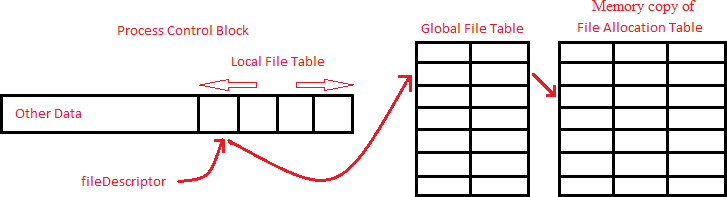
\includegraphics[scale=0.65]{pics/access_method}
	\caption{Diagram showing the method of accessing FAT entry}
	\label{access_scheme}
\end{figure}

\subsection{INT 4}
The file system call \textit{Write} invoke INT 4. INT 4 handles these system calls as follows.

\textbf{Write :} This system call is used to write data into an open file. \\
Syntax : \texttt{int Write(fileDescriptor, mem\_loc, numWords)} 
\footnote{It is advisable to have  a maximum of 1 block for any data file if it has to be modified using \texttt{write} system call since if the modification spans multiple blocks the entire procedure to access a block (outlined above) has to be repeated.} \\
Syscall no : \counter{syscall}
\index{File System Calls!Write}
\begin{itemize}
	\item First of all, the basic block of the file specified by the \texttt{fileDescriptor} is loaded into the scratchpad. This is done in the following way:
	\begin{itemize}
		\item The \texttt{fileDescriptor} is used first to access the local file table entry of the file. An appropriate error is returned if the \texttt{fileDescriptor} is out of the range specified.
		\item This local file table entry is then used to access the global file table entry of the file.
		\item Then the FAT index field in the global file table entry is used to access the FAT entry of the file.
		\item The basic block address present in the FAT entry is then used load the basic block (containing block list and file header info) into the scratchpad. Refer figure~\ref{access_scheme}.
	\end{itemize}	
	
	\item The lseek position present in the GFT entry and \texttt{numWords} are used to index the block list in the basic block to find the block numbers of the block(s) to be written into. \footnote{The data block to which the lseek position is pointing to is got by dividing lseek by the block size. \\
	The data block number calculated above is used to index the block list in the basic block to get the exact location of the data block in the disk. The data block is then loaded from the disk into the scratchpad. \\
	If the words to be read are split across multiple data blocks, the above procedure is repeated.}
	
	\item Each time the block to be written into is loaded into the scratchpad before performing the write operation.
	
	\item After loading the specified block, the content to be written is copied from the user memory location (\texttt{mem\_loc}) into this block. If \texttt{mem\_loc} is out of the address space of the process, an appropriate error code is returned.
	
	\item If the write operation exhausts all the currently allocated blocks, new blocks are allocated as required. This is done in the following way.
	\begin{itemize}
		\item The memory copy of the disk free list \index{Disk Free List!Memory copy} is used to get the block number of a free block.
		\item A new basic block entry is created using this free block number and added to the block list of the basic block. Successive write operations are then performed the usual way.
	\end{itemize}
	
	\item Once all the write operations are over for that block, it is stored back into the disk.
	
	\item The updated copies of FAT \index{File Allocation Table!Memory copy} and disk free list 
	\index{Disk Free List!Memory copy} in the memory are committed to the disk.
	
	\item The return value of this system call is the number of words successfully written. In case of an error, an appropriate error code is returned.
\end{itemize}

\chapter{Multiprogramming}
\label{chp:multiprog}
To support multiprogramming in the system, the kernel makes use of the \emph{scheduler} which is present in the interrupt service routine INT 0\footnote{Unlike other interrupts, INT 0 is called by the machine and not by the user program.}.

\section{Scheduler}
\label{chp:scheduler}
\index{Scheduler}
Whenever a timer interrupt occurs, the kernel temporarily halts the execution of the currently executing process and invokes INT 0.
Refer book~\cite{Crowley} for more details.
Following are functionalities of the scheduler:
\begin{itemize}
	\item If a process is currently running, the scheduler saves the values of all the registers into the corresponding fields in the PCB of that process.
	\item The scheduler scans the ready list starting from the current PID and checks for the presence of a process other than the INIT process.\footnote{This can be accomplished by setting the PID of INIT process as 0 and searching only the entries from 1--11 in the ready list.} If one such process is found, the PID is updated with the index of this entry in the ready list. If no such process is found, then the PID is set to the index of the INIT process in the ready list. Then all the registers of the machine are initialised with their corresponding values obtained from the PCB of the process specified by this PID.
	\item The process switches from \textit{Kernel mode} to \textit{User mode}.
\end{itemize}

\chapter{Process System Calls}
\label{chp:process_system_calls}
\index{Process System Calls}

\section{Process System Calls}
\label{procsyscall}
\index{Process System Calls}
\textit{Process system calls} are used by a process when it has to duplicate itself, execute a new process in its place or when it has to terminate itself. There are three process system calls. An interrupt is associated with each system call. All the necessary arguments for a system call are available in the user stack with the system call number as the last argument.\\

\noindent Interrupt specifications for different \textit{Process system calls} are as follows:

\subsection{INT 5}
The process system call \textit{Fork} invokes INT 5. INT 5 handles these system calls as follows.

\textbf{Fork :}  This system call is used to create a new process having the same code area, data area and list of open files as that of the process which invoked this system call.

The new process that is created is known as the \emph{child} process, and the process which invoked this system call is known as its \emph{parent}.

The register values in the PCB of the child process are initialized with the current register contents.\\
Syntax : \texttt{int Fork()} \\
Syscall no : \counter{syscall}
\index{Process System Calls!Fork}
\begin{itemize}
	\item A vacant entry is searched for in the \emph{Ready list}.
	\item If no entry is found, in the case when there are already 12 processes that are active, an appropriate error code is returned.
	\item The index of this vacant ready list entry is the PID for the child process that is created.
	\item The PID entry in the PCB of the child process is updated with this new PID.
	\item All the registers (except PID) and the local file table of the parent process is replicated in the PCB of the child process.
	\item The code pages, the data page and the stack page of the parent process is replicated for this child process.
	\item The control is returned back to the parent process.
	\item The return value of this system call is the PID of the child process.
\end{itemize}

\subsection{INT 6}
The process system call \textit{Exec} invokes INT 6. INT 6 handles these system calls as follows.

\textbf{Exec :}  This system call is used to load the program, whose name is specified in the argument, in the memory space of the current process and start its execution .\\
Syntax : \texttt{int Exec(filename)} \\
Syscall no : \counter{syscall}
\index{Process System Calls!Exec}
\begin{itemize}
	\item The entire process area of the currently executing process is replaced by that of the program specified in the argument (\texttt{filename}). 
	\item If the file specified by \texttt{filename} is not an executable \footnote{Executables in {\ESIM} must end with an extension \texttt{.sim}} then, an appropriate error code is returned.
	\item The memory copy of the FAT \index{File Allocation Table!Memory copy} is searched to get the location of the basic block of the file specified by \texttt{filename}, which is then loaded into the scratchpad.
	\item This is then used to get the location in the disk of the blocks of the file to be loaded.
	\item The 2 code blocks and 1 data block of the file are loaded from the disk into the corresponding locations in the memory of the code blocks and data block of the current process.
	\item The PCB of the current process is modified to hold the values for that of the new process. The PID and page table, however, remains unchanged.\footnote{This is because the mappings remain the same as the code blocks and data block of the specified executable are loaded into the same locations as of the current process. Since, no new process table entry is created, the PID also remains the same.}
	\item The return value of this system call is 1 in case of a failure. Nothing is returned in case of a success.
\end{itemize}

\subsection{INT 7}
The process system call \textit{Exit} invokes INT 7. INT 7 handles this system call as follows.
\textbf{Exit :}  This system call is used to terminate the execution of the process which invoked it and removes it from the memory . It loads the next available process.\\
Syntax :  \texttt{Exit()}  \\
Syscall no : \counter{syscall}
\index{Process System Calls!Exit}
\begin{itemize}
	\item The entire address space of the currently executing process is set free by setting a value 0 in the memory free list corresponding to the pages occupied by that process.
	
	\item The local file table is traversed and the global file table entry is removed.
	
	\item The ready list entry corresponding to this process is set to zero thereby releasing all the data structures used by the process (fig~\ref{fig:ds with process}).
	
	\item The ready list is then searched for the next available process. The INIT process is excluded in this search.\footnote{This can be accomplished by setting the PID of INIT process as 0 and searching only the entries from 1--11 in the ready list.} If one such process is found, the PID is updated with the index of this entry in the ready list. If no such process is found, then the PID is set to the index of the INIT process in the ready list.
	
	\item All the registers of the machine are initialised with their corresponding values obtained from the PCB of the process specified by the new PID.
	
	\item The process switches from \textit{Kernel mode} to \textit{User mode}.
\end{itemize}

\section{INIT Process}
The INIT process is the first user process loaded by the OS on the OS startup. INIT was previously defined in chapter~\ref{chp:osstartup} as a normal user program. Since multiprogramming functionalities have been added to the OS, INIT must be modified. The modified specification of INIT process is as follows:
\begin{itemize}
	\item  It provides an interface for the users to run other user programs.
	\item The user enters the name of a valid executable file (which should be made available in the disk) in the shell. If the specified file is not found, an appropriate error code is returned.
	\item If the specified executable file is found, the INIT process forks and does exec on the that file.
	\item Entering the keyword HALT instead of the name of an executable file invokes the Shutdown system call.
\end{itemize}

All the user processes other than INIT are added to entries 1-11 of the ready queue keeping the 0th entry (corresponding to INIT) untouched. INIT loads the first process and thereafter all context switches occur among the other processes in the ready queue. INIT is switched back only when the ready queue (entries 1-11) is free so that the user can load another executable file via the shell. 

%\appendix TODO !!
%\section{Simple Integer Machine (SIM) architecture}
% \chapter{System Programmer's manual}
% The following diagram illustrates the interaction among various modules that have been written in the code. 
% 
%  \begin{figure}[htp!]
% 	  \centering
% % 	  \includegraphics[scale=0.55]{pics/spm}
% 	  \caption{Interaction among various modules in the implementation}
% 	  \label{fig:spm}
% 	  \end{figure}
% 
% Each module performs a specific function which has been well documented in the code. All variables and data structures that are used are suitably named and proper constants have been defined for anything that has a fixed value like location in memory of the various data structures and other machine constants. 


\chapter{Future Work}
\label{futurework}

In the project so far we have documented the machine and the operating system. However there is no step-by-step instruction for the student showing him the way he has to proceed for designing the operating system. This roadmap is intended to do the same.\\

The current machine supports both integer and string data type. However the registers can hold only integers. these have led to various problems while implementing the operating system. One such problem is the non availability of using predefined strings in kernel code. Converting the current machine to a pure \emph{String} machine will solve this problem.\\

The project was developed as a means for replacing NACHOS. To reach out to a wider audience it would be better to host this on a public domain which would be accessible to teachers and students.\\

Since the student is working directly on the machine and developing the operating system from scratch, it is advisable to have a more advanced debugging interface.\\

Finally the deployment of the finished tool in Operating system Lab.

\chapter{Conclusion}
\label{chp:conclusion}
\index{Conclusion}

The entire project was started as a way for increasing the knowledge gained by a student taking Operating System lab. The current lab utilizes NACHOS~\cite{nachos} and students gain little knowledge from it. Moreover the clerical overhead involved in implementing an Operating System on NACHOS is way more than the knowledge gained from it.

The current project was done taking in mind the difficulties that were faced while using NACHOS. It was designed in a way so as to minimize the clerical overhead and give the student a feel of how an Operating System functions. How successful we have been, only time can tell. However from our experience we feel that this new project is above NACHOS in terms of conceptual knowledge gained and ease of use.

There have been some decisions which deviate from how an Operating System works. This includes fixing the location of INIT process and Exec not checking whether the new file to load is an executable or not. These problems arose because the Kernel codes do not have a stack. One solution was to do what we did and another one was to add a kernel stack. The latter would have involved changes in design and so we did not choose it. We expect this to be solved in the next version of the project where the entire machine would have only string data type.

Writing an Operating System is not so tedious on this machine  as it was in NACHOS. We had to write an Operating System for testing and debugging. From that experience, we can clearly say that the student in fact learns not only a lot about Operating System but also many new other concepts. One such concept is the use of memory de-referencing.

On an overall note, the project has ended on a high. Though it has its faults, it is better than the tool currently being utilized. The next version, if it goes as planned, will take it a level higher. Nevertheless we feel that what we have done is ready to be put forth before the student community to aide them in learning Operating Systems.

\appendix
%\documentclass[11pt]{article}
%\usepackage{tabularx}
%\usepackage{listings}
%\usepackage{verbatim}
%\usepackage[bookmarks]{hyperref}
%
%
%\title{SPSIL \\ Language Specification \\
%Version 1.0}
%\author{Dr. K. Muralikrishnan  \\ \texttt{kmurali@nitc.ac.in} \\ {NIT Calicut} }
%
%
%\hypersetup{
%colorlinks=false,
%urlcolor=cyan,
%pdfborder= 0 0 0
%}
%
%
%\begin{document}
\chapter{SPSIL}
 \newcommand{\kw}[1]{\texttt{#1}}

%.......................Title Page.................................>%
%\maketitle

%\pagebreak
%......................Table of Contents............................%
\thispagestyle{plain}

%\tableofcontents
%\pagebreak

%...............................Introduction..........................%

\section{Introduction}
\paragraph{}
\textit{SPSIL} or \textit{System Programmer's Simple Integer Language} is an untyped programming language designed for implementation of an operating system on ESIM \textit{(Extended Simple Integer Machine)} architecture. The language is minimalistic and consists only of basic constructs required for the implementation. Programming using SPSIL requires a  basic understanding of the underlying ESIM architecture and operating system concepts. 



%-----------------------------Lexical Elements-------------------------%
\section{Lexical Elements}




%*********%
\subsection{Comments and White Spaces}

SPSIL allows only single line comments. Comments start with the character sequence \textbf{//} and stop at the end of the line. 
White spaces in the program including tabs, newline and horizontal spaces are ignored.


%*********%
\subsection{Keywords}
The following are the reserved words in SPSIL and it cannot be used as identifiers.

\begin{tabular}{c c c c c }
\kw{alias} 		& 	\kw{else} 		& 	\kw{if} 		&    \kw{store} 	&   \kw{while}     \\
\kw{define} 	& 	\kw{endif}  	& 	\kw{ireturn} 	&	 \kw{strcmp}  	&  \kw{continue}\\
\kw{break}      & \kw{do}  		&   \kw{endwhile} 	& 	\kw{load} 		&	\kw{then} 	
\end{tabular}




%*********%
\subsection{Operators and Delimiters}

The following are the operators and delimiters in SPSIL   \\

\begin{tabular}{c c c c c c c c c c c c }
( 		 			& 		) 		& 			;		 &			[		&		 ]    &
/		 			& 		*		 & 		+ 		 & 		-  		& 		\% 		  \\
\textgreater  		& 	   \textless   &  \textgreater = 	 &  \textless =	&	    !=		&	==	  &	=  &  \&\&  	  &		$\Vert$	&	!	\\
\end{tabular}


%*********%
\subsection{Registers}
SPSIL allows the use of 20 registers for various operations.(R0-R7, S0-S7, BP, SP, IP, PID)

%*********%
\subsection{Identifiers}
Identifiers are used as symbolic names for constants and aliases for registers. Identifiers should start with an alphabet but may contain alphabets, digits and/or underscore (\_). No other special characters are allowed in identifiers.  

%*********%
\subsection{Literals}
Only integer literals are permitted in SPSIL. An integer literal is a sequence of digits representing an integer. Negative integers are represented with a negative sign preceding the sequence of digits.  



%-----------------------------Registers-------------------------%%
\section{Register Set}

SPSIL doesn't allow the use of declared variables. Instead a fixed set of registers is provided. The register set in SPSIL contains 20 registers. There is a direct mapping between these registers and the machine registers in ESIM.   \\

\begin{center}
\begin{tabular}{| c | c | }
\hline
R0-R7 & Program Registers \\
\hline
S0-S7 & Kernel Registers \\
\hline
BP 		& Base Pointer \\
\hline
SP		& Stack Pointer \\
\hline
IP		& Instruction Pointer \\
\hline
PID	& Process Identifier \\
\hline
\end{tabular}
\end{center}

\subsection{Aliasing}
Any register can be referred to by using a different name. A name is assigned to a particular register using the \textbf{alias} keyword. Each register can be assigned to only one alias at any particular point of time. However, a  register can be reassigned to a different alias at a later point. Aliasing can also be done inside the \textbf{if} and \textbf{while} block. However, the alias will only be valid within the if and while block it is defined in. The already defined alias for the register(if any) will only be hidden inside if and while blocks. No two registers can have the same alias name simultaneously.



%-----------------------------Constants-------------------------%%
\section{Constants}
Symbolic names can be assigned to values using the \textbf{define} keyword. Unlike aliasing, two or more names can be assigned to the same value. A constant can only be defined once in a program.
	
\subsection{Predefined Constants}
SPSIL provides a set of predefined constants. These predefined constants can be assigned to different values explicitly by the user using \textbf{define} keyword. These constants are mostly starting addresses of various OS components in the memory.

The predefined set of constants provided in SPSIL are \\
\begin{center}
\begin{tabular}{| c | c |}
\hline
\textbf{Name} & \textbf{Default Value} \\
\hline
SCRATCHPAD 	& 	256 \\
\hline
PAGE\_TABLE 	& 	512  \\
\hline
MEM\_LIST 	&	576 	\\
\hline
FILE\_TABLE 	& 	640		\\
\hline
READY\_LIST 	& 	736	\\
\hline
PROC\_TABLE 	& 	767 \\
\hline
FAT 		& 	1024    \\
\hline
DISK\_LIST 	& 	1536 	\\
\hline
USER\_PROG 	& 	1792	\\
\hline
INTERRUPT & 	13824	\\
\hline
\end{tabular}
\end{center}


%----------------------------Expressions-------------------------_%
\section{Expressions}
An expression specifies the computation of a value by applying operators to operands. SPSIL supports arithmetic and logical expressions.

\subsection{Arithmetic Expressions}

Registers, constants, and 2 or more arithmetic expressions connected using arithmetic operators are categorized as arithmetic expressions. SPSIL provides five arithmetic operators, viz., +, -, *, / (Integer Division) and \% (Modulo operator) through which arithmetic expressions may be combined. Expression syntax and semantics are similar to standard practice in programming languages and normal rules of precedence, associativity and paranthesization hold. 


\subsection{Logical Expressions}

Logical expressions may be formed by combining arithmetic expressions using relational operators. The relational operators supported by SPSIL are \begin{verbatim}  <, >, <=, >=, ==, !=
\end{verbatim}
Standard  meanings apply to these operators. A relational operator will take in two arguments and return 1 if the relation is valid and 0 otherwise. Logical expressions themselves may be combined using logical operators, \&\& (logical and) ,  $\Vert$ (logical or) and ! (not).

\subsection{String Comparison}
The only operation that can be performed on strings stored in memory is string camparison. \textbf{strcmp} is used to compare two strings whose address is stored in the registers that are given as operands. \\

 e.g. \textit{strcmp(R2,R5)}


\subsection{Addressing Expression}
Memory of the meachine can be directly accessed in an SPSIL program. A word in the memory is accessed by specifying the addressing element, i.e. memory location within [ ]. This  corresponds to the value stored in the given address. An arithmetic expression or an addressing expression can be used to specify the address. \\

Examples of addressing expressions: \\\   
 [1024], [R3], [R5+[S7]+128], [FAT + (PID*16) + S2] etc.

%-----------------________Statements---------------------------_%
\section{Statements}

Statements control the execution of the program. All statements in SPSIL are terminated with a semicolon ;



\subsection{Define Statement}
Define statement is used to define a symbolic name for a value. Define statements should be  used before any other statment in an SPSIL program. The keyword \textbf{define} is used to associate a literal to a symbolic name. \\

\textit{ \textbf{define} constant\_name value; }


\subsection{Alias Statement}
An \textbf{alias} statement is used to  associate a register with a name. \textbf{Alias} statements can be used anywhere in the program except within \textbf{if} and \textbf{while} statements.\\

\indent \textit{ \textbf{alias}  alias\_name register\_name ;} \\


\subsection{Assignment Statement}
The SPSIL assignment statement assigns the value of an  expression or value stored in a memory address to a register or a memory address. \textbf{=} is the assignment operator used in SPSIL. The operand on the right hand side of the operator is assigned to the left hand side. The general syntax is as follows \\

\indent \textit{ Register / Alias / [Address] = Expression / [Address] ;}

\subsection{strcpy Statement}
The SPSIL \textbf{strcpy} statement copies a string in one memory location to another memory location. Registers which store the  memory location of the destination and the source are given as R{\tiny d} and R{\tiny s} respectively.\\
\indent \textit{ \textbf{strcpy}(R{\tiny d}, R{\tiny s});}

\subsection{If Statement}
\textbf{If} statements specify the conditional execution of two branches according to the value of a logical expression. If the expression evaluates to 1, the \textbf{if} branch is executed, otherwise the \textbf{else}  branch is executed. The \textbf{else} part is optional. The general syntax is as follows  \\

\textit{
\textbf{if} (logical expression) \textbf{then}  \\
 \indent \indent statements; \\
\indent \textbf{else} \\
\indent  \indent statements; \\
\indent \textbf{endif;}  \\
}



\subsection{While Statement}
\textbf{While} statement iteratively executes a set of statements based on a condition. The condition is defined using a logical expression.  The statements are iteratively executed as long as the condition is true.\\

\textit{
\textbf{while} (logical expression) \textbf{do}  \\
 \indent \indent statements; \\
\indent \textbf{endwhile;}  \\
}


\subsection{Break statement}
\textbf{Break} statement is a statement which is used in a while loop block. This statement stops the execution of the loop in which it is used and passes the control of execution to the next statement after the loop. This statement cannot be used anywhere else other than while loop. The syntax is as follows\\

\textit{\textbf{break} ;}


\subsection{Continue statement}
\textbf{Continue} statement is a statement which is also used only in a while loop block. This statement skips the current iteration of the loop and passes the control to the next iteration after checking the loop condition. The syntax is as follows\\

\textit{\textbf{continue} ;}

\subsection{ireturn Statement}
\textbf{ireturn} statement is used to pass control from kernel mode to user mode. The \textbf{ireturn} is generally used at the end of an interrupt code.

\textit{\textbf{ireturn};}


\subsection{Load / Store Statements}
Loading and storing between filesystem and memory is accomplished using \textbf{load} and \textbf{store} statements in SPSIL. \textbf{load} statement loads the block specified by \textit{block\_number} from the disk to the the page speficied by the \textit{page\_number} in the memory. \textbf{store} statement stores the page specified by \textit{page\_number} in the memory to the the block speficied by the \textit{block\_number} in the disk. The page number and block number can be specified using arithmetic expressions.

\textit{\textbf{load} (page\_number, block\_number);}

\textit{\textbf{store} (page\_number, block\_number);}


%\end{document}

%\documentclass[11pt]{article}
%\usepackage{booktabs}
%\usepackage{fullpage}
%\usepackage{palatino}
%\usepackage{tabularx}
%\usepackage{listings}
%\usepackage{verbatim}
%\usepackage[bookmarks]{hyperref}
%
%
%\title{APSIL \\ Language Specification \\
%Version 1.0}
%\author{Dr. K. Muralikrishnan  \\ \texttt{kmurali@nitc.ac.in} \\ {NIT Calicut} }
%
%
%\hypersetup{
%colorlinks=false,
%urlcolor=cyan,
%pdfborder= 0 0 0
%}
%
%
%\begin{document}
\chapter{APSIL}
%\newcommand{\kw}[1]{\texttt{#1}}

%.......................Title Page.................................>%
%\maketitle

%\pagebreak
%......................Table of Contents............................%
\thispagestyle{plain}

%\tableofcontents
%\pagebreak

%...............................Introduction..........................%

\section{Introduction}
\paragraph{}
\textit{APSIL} or \textit{Application Programmer's Simple Integer Language} is a simple and strongly typed programming language. The features and constructs of this language are minimal and mainly intended for testing an experimental operating system. The compiler of APSIL runs on ESIM (\textit{Extended Simple Integer Machine}) architecture.
\paragraph{}
This document describes briefly describe the programming constructs, syntax and semantics APSIL. The structure of APSIL is similar in some aspects to programming languages like C and Java. 

A typical APSIL program is orgnaized in the following way. 

\begin{verbatim}
Global Declarations
...
Function Definitions
...
Main Function
\end{verbatim}


%-----------------------------Lexical Elements-------------------------%
\section{Lexical Elements}




%*********%
\subsection{Comments and White Spaces}

APSIL allows only line comments. Line comments start with the character sequence \textbf{//} and stop at the end of the line. 
White spaces in the program including tabs, newline and horizontal spaces are ignored.




%*********%
\subsection{Keywords}
The following are the reserved words in APSIL and it cannot be used as  identifiers.

\begin{tabular}{c c c c c c }
\kw{read} & \kw{write} & \kw{if} &   \kw{then} &   \kw{else} &   \kw{endif} \\
\kw{while} &   \kw{do} &   \kw{endwhile} &  \kw{break} & \kw{continue} & \kw{integer} \\
\kw{string} & \kw{main} & \kw{return} &    \kw{decl} &		\kw{enddecl}  &  \kw{Create}  \\
\kw{Open} &   \kw{Write} & \kw{Seek}  & \kw{Read} & \kw{Close} &   \kw{Delete}    \\
\kw{Fork} & \kw{Exec} & \kw{Exit} 
\end{tabular}




%*********%
\subsection{Operators and Delimiters}

The following are the operators and delimiters in APSIL   \\

\begin{tabular}{c c c c c c c c c c c c c}
( 		 & 		) 		& 		\{		 &		\} 		& 		[		&		 ]    &
/		 & 		*		 & 		+ 		 & 		-  		& 		\% 		  \\
\textgreater  & 	   \textless   &  \textgreater = 	 &  \textless =	&	    !=		&	==	  
  & 		;	&	=  &  \&\&  	  &		$\Vert$	&	!	\\
\end{tabular}




%*********%
\subsection{Indentifiers}

Identifiers are names of variables and user-defined functions. Identifiers should start with an alphabet, and may contain both alphabets and digits. Special characters are not allowed in identifiers.
\begin{verbatim}
identifier -> (alphabet)(alphabet | digit)*
\end{verbatim}




%*********%
\subsection{Literals}
There are integer literals and string literals in APSIL. An integer literal is a sequence of digits representing an integer.
Negative integers are represented with a negative sign preceding the sequence of digits. Any sequence of characters enclosed within double quotes (") are considered as string literals. However APSIL restricts string literals to size of atmost 16 characters including the '\textbackslash 0' character which is implicitly appended at the end of a string value. 
\\
\\
Examples of literals are \texttt{
 19, -35, "Hello World"}


%-----------------------------Data Types-------------------------%
\section{Data Types}

\subsection{Primitive Types}
There are two primitive datatypes in APSIL. 
\begin{enumerate}

\item \textbf{Integer} : An integer value can range from -32767 to +32768. An integer type variable is declared using the keyword \kw {integer}
\item \textbf{String}  
A string type represents the set of string values. A string value can be atmost 16 characters long. String type variables is declared using the keyword \kw{string}.
\end{enumerate}


\subsection{Arrays}
Arrays are  sequence of elements of a single type. Arrays can be of \textbf{integer} or \textbf{string} data types.
APSIL allows the use of single-dimensional arrays only, i.e. linear arrays. Array elements are accessed by the array name followed an index value within square brackets ( e.g. arr[10] ).


%-----------------------------Declarations and Scope-------------------------%%
\section{Declarations and Scope}

Declarations should be made for  variables and functions defined in the APSIL program.




\subsection{Global Variables}
Global variables are declared in the first section of the program within a \textbf{decl} ... \textbf{enddecl} block. Global variables can be accessed from any function in the program. Global variables can be of integer, string, integer array or string array datatypes. Global variables are declared with its datatype followed by the variable name. If the variable refers to an array the size of the array must be given in square brackets. The general form of declarations is as follows 

\textit{type variable\_name;} 

\textit{type variable\_name[size];}





\subsection{Function Declaration}
For every function except the \textbf{main()} function defined in a APSIL program, there must be a declaration. All functions have global scope and is declared in the first section within  \textbf{decl} ... \textbf{enddecl} block, along with the global variables.

A function declaration should specify the name of the function, the name and type of each of its arguments and the return type of the function. A function can have integer/string arguments. Parameters may be passed by value or reference. Arrays cannot be passed as arguments. If a global variable name appears as an argument, then within the scope of the function, the new declaration will be valid and global variable declaration is suppressed. Different functions may have arguments of the same name. For arguments that are passed by reference, the argument name is preceded by an ampersand(\&) in the function declaration. The return type of a function must be either integer or string. The general form of declarations is as follows \\ 

\textit{type function\_name (type1 argument1,argument2,...; type2 argument1,argument2,...;...);}
\\
\\
Examples for global declarations
\begin{lstlisting}
decl
	integer x,y,a[10],b[20];	
	integer f1(integer a1,a2; string b1; integer &c1), f2(); 
	string t, q[10], f3(integer x); 
	integer swap(integer &x, &y);	 
enddecl
\end{lstlisting}





\subsection{Local Variables}
Local variables can be declared anywhere inside a function definition except in the body of \textbf{if} and \textbf{while}. Local variables will have a function scope, i.e. it can only be accessed in the function in which it is declared. Arguments of a function are treated as local variables. Local variables can be integer or string. Arrays cannot be declared locally. All globally declared variables are visible inside a function, unless suppressed by a re-declaration. The general form of declarations is as follows \\

\textit{type variable\_name;} 





%------------------__Function Definition----------------------_%

\section{Function Definition and Main Function}

Every APSIL program must have a \textbf{main()} function and zero or more user-defined functions. Every function other than the \textbf{main()} function must be declared within the \textbf{decl ... enddecl} block. The general form of a function definition is given below 
\\
\\
\textit{
type function\_name(ArgumentList) \\ \{ \\
  Function Body \\
\}
}
\\
\\
The function body must contain a return statement and the return value must be of the return type of the function. The arguments and return type of each function definition should match exactly with the corresponding declaration. Every declared function must have a definition. The signature of the function in the delcaration should match the definition of the function which includes the return type, and the names, passing mehtod and datatypes of the arguments. The language supports recursion and static scope rules apply.




\subsection{main()}
The \textbf{main()} function must be a zero argument function of type integer. Program execution begins from the body of the \textbf{main()} function. The \textbf{main()} function need not be declared. The \textbf{main()} function definition follows all user-defined function definitions.  The definition part of \textbf{main()} should be given in the same format as any other function.



%----------------------------_Expressions-------------------------_%
\section{Expressions}
An expression specifies the computation of a value by applying operators and functions to operands. Function call in APSIL are treated as expressions, and the value of the expression is its return value. APSIL supports arithmetic and logical expressions



\subsection{Arithmetic Expressions}

Any integer value, variable, function returning an integer or 2 or more arithmetic expressions connected by arithmetic operators termed as arithmetic expressions. APSIL provides five arithmetic operators, viz., +, -, *, / (Integer Division) and \% (Modulo operator) through which arithmetic expressions may be combined. Expression syntax and semantics are similar to standard practice in programming languages and normal rules of precedence, associativity and paranthesization hold. APSIL is strongly typed, and hence the types of the oprands must match the operation. 


\subsection{Logical Expressions}

Logical expressions may be formed by combining arithmetic expressions using relational operators. The relational operators supported by APSIL are \begin{verbatim}  <, >, <=, >=, ==, !=
\end{verbatim}
Standard  meanings apply to these operators. The operators take two arithmetic expressions as operands and the result will be a boolean value, either of 1(true) or 0(false). Only realational operator that can be applied to two strings is == (to check equality). This also considered as a Logical expression. Logical expressions themselves may be combined using logical operators, \&\& (logical and) ,  $\Vert$ (logical or) and ! (not).

\subsection{Function Call}

All functions except the \textbf{main()} function can be invoked from any other function including itself. The general form of a function call is \\

\textit{function\_name(value1,value1...);}
\\

Function calls are treated as expressions. The function takes in the values of its arguments and returns a value of type equal to the return type of the function. This value is treated as the evaluated result of the function call.




%-----------------________Statements---------------------------_%
\section{Statements}

Statements control the execution of the program. All statements in APSIL are terminated with a semicolon ;





\subsection{Assignment Statement}
The APSIL assignment statement assigns the value of an expression to a variable, or an indexed array of the same type or a string value to a string variable. \textbf{=} is known as the assignment operator. Initialization during declaration is not allowed in APSIL. The general syntax is as follows \\
\textit{ variable\_name = string\_value / array\_variable / expression }






\subsection{If Statement}
\textbf{If} statements specify the conditional execution of two branches according to the value of a boolean expression. If the expression evaluates to true, the \textbf{if} branch is executed, otherwise, if present, the \textbf{else}  branch is executed. The \textbf{else} part is optional. The general syntax is as follows  \\

\textit{
\textbf{if} (logical expression) \textbf{then}  \\
 \indent \indent statements; \\
\indent \textbf{else} \\
\indent  \indent statements; \\
\indent \textbf{endif;}  \\
}



\subsection{While Statement}
\textbf{While} statement iteratively executes a set of statements based on a condition which is a logical expression.  The statements are iteratively executed as long as the logical expression evaluates to true.

\textit{
\textbf{while} (logical expression) \textbf{do}  \\
 \indent \indent statements; \\
\indent \textbf{endwhile;}  \\
}

\subsection{Break statement}
\textbf{Break} statement is a statement which is used in a while loop block. This statement stops the execution of the loop in which it is used and passes the control of execution to the next statement after the loop. This statement cannot be used anywhere else other than while loop. The syntax is as follows\\

\textit{\textbf{break} ;}

\subsection{Continue statement}
\textbf{Continue} statement is a statement which is also used only in a while loop block. This statement skips the current iteration of the loop and passes the control to the next iteration after checking the loop condition. The syntax is as follows\\

\textit{\textbf{continue} ;}



\subsection{Return statement}
\textbf{Return} statement in a function passes the control from the callee to the caller function and returns a value to the caller function. All functions including the \textbf{main()} must have exactly one \textbf{return} statement and it should be the last statement in the funtion body. The return type of the function should match the type of the expression. The return type of main is integer. The syntax is as follows\\

\textit{\textbf{return} expression;}


\subsection{Read/Write statements}
The standard input and output statements in APSIL are \textbf{read} and \textbf{write} respectively. The read statement reads an integer value from the standard input device into an integer variable or an indexed array variable or a string value into a string variable. The write statement outputs a string literal or the value of string variable or an arithmetic expression  into the standard output.\\

\textit{\textbf{read} variable\_name;}

\textit{\textbf{write} expression / string;}






\section{System Calls}

System Calls allow the programs written in APSIL to interact with the operating system running on the ESIM architecture. 10 System Calls are supported by APSIL. 




\subsection{Create}
Creates a file with the specified filename in the filesystem. The return value of this system call is 0 in case of success and the appropriate error code in case of failure.
\\

\textit{integer \textbf{Create}(string filename);}






\subsection{Open}
Returns a file descriptor of the file in the filesystem with the specified filename. The file descriptor is an integer value. If the \textbf{Open} fails, an appropriate error code is returned.
.\\

\textit{integer \textbf{Open}(string fileName);}





\subsection{Read}
Reads the specified number of words(16 bytes) from a file which has the specified file descriptor into a string array. The return value of this system call is the number of words successfully read. If the \textbf{Read} fails, an appropriate error code is returned.\\

\textit{integer \textbf{Read}(integer fileDescriptor, string buffer[], integer numWords);}





\subsection{Write}
Writes the specified number of words from the string buffer to a file in the filesystem with the specified file descriptor. The return value of this system call is the number of words successfully written. If the \textbf{Write} fails, an appropriate error code is returned.\\

\textit{integer \textbf{Write}(integer fileDescriptor, string buffer[], integer numWords);}





\subsection{Seek}

\textbf{Seek} is used to change the read/write head position in a file. It moves the head to the specified number of words from the beginning of the file. The return value of this system call is 0 in case of success and the appropriate error code in case of failure.\\

\textit{integer \textbf{Seek}(integer fileDescriptor, integer numWords);}
 
 
 
 
 \subsection{Close}
This system call is used to close an open file. The return value of this system call is 0 in case of success and the appropriate error code in case of failure.\\

\textit{integer \textbf{Close}(integer fileDescriptor);}




\subsection{Delete}
This system call is used to delete the file from the file system whose name is specified in the
argument. The return value of this system call is 0 in case of success and the appropriate error code in case
of failure.\\

\textit{integer \textbf{Delete}(string fileName);}



\subsection{Fork}
This system call is used to create a copy of the current process in the system. The return value of this system call is the PID of the child process for the parent, and 0 for the child.


\textit{integer \textbf{Fork}();}




\subsection{Exec}
This system call is used to load the program, whose name is specified in the argument, in the
memory space of the current process and start its execution. The return value of this system call is 1 in case of failure.
\textit{integer \textbf{Exec}(string fileName);}




\subsection{Exit}
This system call is used to terminate the execution of the process which invoked it and remove it from the memory.

\textit{void \textbf{Exit}();}


\subsection{Halt}
This system call is used to halt the machine.

\textit{void \textbf{Halt}();}

%\end{document}


\clearpage
\addcontentsline{toc}{chapter}{Index}
\printindex

\clearpage
\phantomsection
\addcontentsline{toc}{section}{Bibliography}
\bibliographystyle{alpha}
\bibliography{references}


\end{document}
%%%% Document ends %%%%%%

% Draft v1.0 : K Dinesh
% Draft v2.0 : Albin Suresh & Ramnath J
